\documentclass{article}
\usepackage{graphicx}
\usepackage[english]{babel}
\usepackage[a4paper,top=2.2cm,bottom=2.2cm,left=3cm,right=3cm,marginparwidth=1.75cm]{geometry}
\usepackage{amsmath}
\usepackage{graphicx}
\usepackage[colorlinks=true, allcolors=blue]{hyperref}
\usepackage{indentfirst}
\usepackage{enumitem}
\usepackage{csquotes}
\usepackage[backend=biber, style=chicago-authordate]{biblatex}
\usepackage{multirow,array}
\addbibresource{ref.bib}
\setlist[itemize]{noitemsep, topsep=0pt}
\usepackage{subfig}




\title{\textbf{Open-ended Exploration Report}}
\author{Haiming Li, Shuxian Chen, Witty Wen}
\date{December 3, 2023}
\begin{document}
\maketitle

\section{Introduction}

In this report, we use the pre-pandemic dataset provided by the National Health and Nutrition Examination Survey (NHANES), covering the period from 2017 to March 2020, to deeply investigate the potential relationships between cholesterol levels and a variety of biomarkers, body measurements, and demographic features. Given the rising prevalence of cardiovascular diseases, cholesterol levels become one of the most important major risk factors, the aim of our study is to reveal the key factors influencing cholesterol levels, thereby offering scientific insights for public health interventions. To achieve this, we employed two machine learning techniques, Support Vector Machine (SVM) and eXtreme Gradient Boosting (XGBoost), optimizing these models through cross-validation and L1/L2 regularization. Furthermore, we used SHAP values (SHapley Additive exPlanations) to compare the feature importance in the SVM and XGBoost models and to explore how these features vary across different age groups. SHAP values provide a means to interpret complex machine learning model decisions, enabling us to quantify each feature's contribution to the model's predictions. By comparing the SHAP values from SVM and XGBoost models, we aspire to gain deeper insights into how different algorithms assess the importance of features and to examine how age factors influence these relationships. The outcomes of this study are anticipated not only to offer new insights into the factors affecting cholesterol levels but also to guide the development of preventive strategies targeted at diverse age groups, thereby contributing to the reduction of overall cardiovascular disease risks. 

\section{Data}

We utilize the 2017-March 2020 Pre-Pandemic Demographics data. The data collection includes multiple datasets, which contain information such as fitness test results, cholesterol levels, blood heavy metal measures, and demographic records. Since the suspended field operations of NHANES programs were stopped in March 2020 due to the pandemic, the part of the dataset collected between 2019 and March 2020 was combined with the data from the 2017-2018 cycle to form a fully representative sample of that period. 

The focus of our research is the relationship between features and cholesterol levels and the difference in the importance of the feature across all age groups, so we utilized the following main variables:

\begin{itemize}
    \item \textbf{LBXTC} (mg/dL): Binary encoding of cholesterol level, 1 for levels $\geq$ 200, otherwise 0.
    \item \textbf{BMXWT} (kg): Body weight.
    \item \textbf{BMXBMI}: Body Mass Index, a nonlinear combination of weight and height.
    \item \textbf{LBXBPB} (ug/dL): Blood lead concentration.
    \item \textbf{LBXBCD} (ug/dL): Blood cadmium concentration.
    \item \textbf{LBXTHG} (ug/dL): Blood mercury concentration.
    \item \textbf{LBXBSE} (ug/dL): Blood selenium concentration.
    \item \textbf{LBXBMN} (ug/dL): Blood manganese concentration.
    \item \textbf{RIDAGEYR} (years): Age.
    \item \textbf{INDFMPIR}: Ratio of family income to poverty.
    \item \textbf{RIAGENDR}: Gender (1: Male, 2: Female).
\end{itemize}

Since these variables come from 4 different datasets, we have joined all of them with the Respondent Sequence Number (SEQN). For the LBXTC variable, since we are performing binary classification, as the response variable of the model, we encode all values greater than 200 as 1, and other values as 0. For other features, we have removed all missing values. Here's a correlation matrix partitioned by the binary label.
\begin{figure}[!ht]
\centering
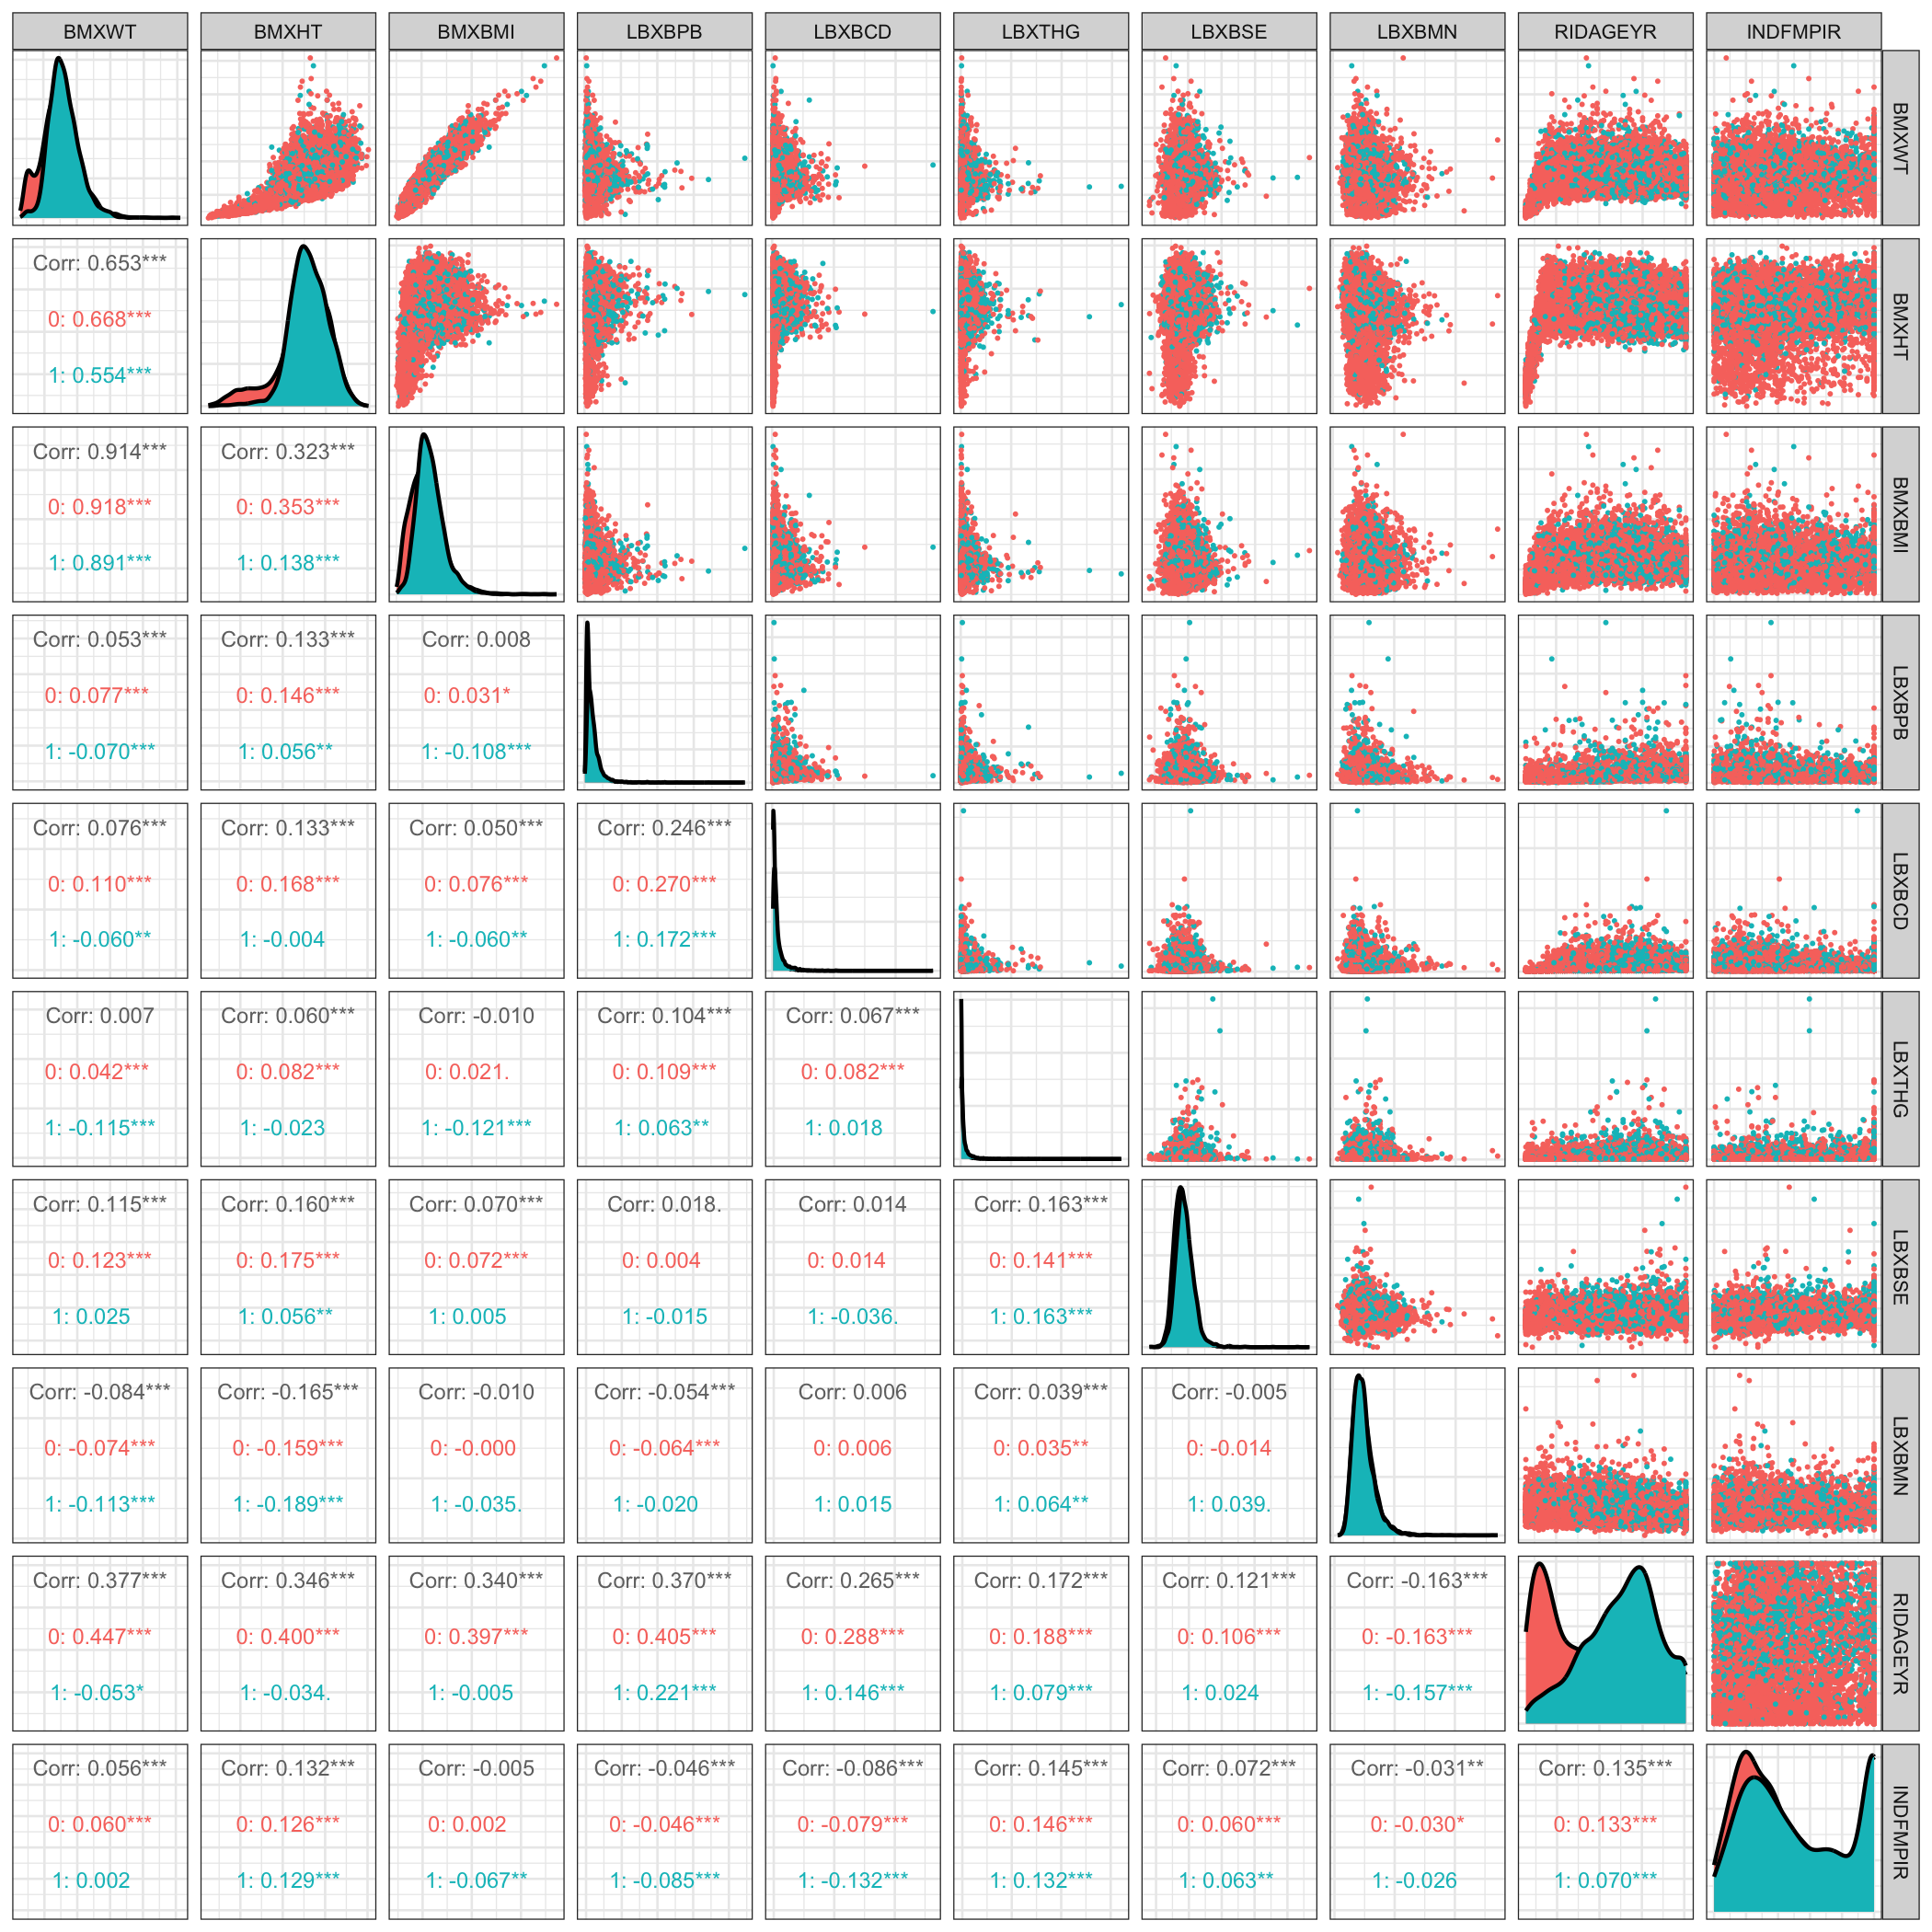
\includegraphics[width=15cm]{data_visual.png}
\caption{Scatter Plot Matrix}
\end{figure}

\noindent Here's a contingency table of cholesterol level binary label v.s. gender.
    \begin{center}
        \begin{tabular}{cc|c|c|c|c|}
          & \multicolumn{1}{c}{} & \multicolumn{3}{c}{$\text{GENDER}$}\\
          & \multicolumn{1}{c}{} & \multicolumn{1}{c}{$1$}
          & \multicolumn{1}{c}{$2$}\\\cline{3-4}
          \multirow{2}*{$\text{LBXTC}$}  
          & $0$ & $3494$ & $3426$ \\\cline{3-4}
          & $1$ & $1064$ & $1302$ \\\cline{3-4}\\
        \end{tabular} 
    \end{center}

\section{Methods}

In our research, we used 4 of the 7 tools requested: lasso/ridge penalties, SVM, trees, and cross-validation. We employed two distinct machine learning algorithms: Support Vector Machine (SVM) and eXtreme Gradient Boosting (XGBoost). The reason we use these two tools is that SVM with radial basis function kernel and XGBoost are common high-performance models that are well suited for our binary classification problem.

For each model, we utilized a five-fold cross-validation approach to optimize the hyperparameters, which ensures the generalizability of the model. We also applied L1/L2(lasso/ridge) penalty in both models to avoid overfitting and thus ensure model performance. After confirming the feature importance based on the shape and variable value, we also modeled the two algorithms we used separately for the data as a whole and for different parts of the data set.

This methodical approach was instrumental in developing robust and reliable binary classification models.

\subsection{Support Vector Machine}

For the optimization of the Support Vector Machine model, we perform hyperparameter tuning using Grid Search with Cross-Validation scoring strategy. This method effectively explores the listed possibilities, and is particularly effective at finding exactly the best hyperparameters for a specified parameter type and range.

The hyperparameters we chose for this model are as follows:

\begin{itemize}
    \item \texttt{C}: From 100 to 200, increment by 1. This parameter controls the trade-off between achieving low error on the training data and minimizing the weight norm. (L2 penalty)
    \item \texttt{gamma}: From $7 \times 10^{-4}$ to $1 \times 10^{-3}$, linear space of 100 elements. This parameter defines how far the influence of a single training example reaches.
\end{itemize}

The grid search process uses 5-fold cross-validation and scoring the models based on their ROC-AUC score. This design can help our models perform better when faced with imbalanced datasets or situations where both precision and recall are critical. After the grid search process is completed, the best estimator is saved for later use.

This comprehensive approach utilizes grid search and carefully selected hyperparameter ranges in the grid to help fine-tune our SVM model, thereby improving its accuracy in predicting the response variable.

\subsection{EXtreme Gradient Boosting}

For the optimization of the XGBoost model, we perform hyperparameter tuning using Randomized Search with Cross-Validation scoring strategy due to the extensive parameter space. This method effectively explores a wide range of possibilities, and is particularly effective for finding optimal hyperparameters in large search spaces.

Hyperparameters are selected from:

\begin{itemize}
    \item \texttt{n\_estimators}: From 5 to 35, increment by 5. This parameter defines the number of boosting rounds or trees to build.
    \item \texttt{max\_depth}: From 3 to 12, increment by 1, controlling the maximum depth for each trees.
    \item \texttt{min\_child\_weight}: From 0.0001 to 0.5, increment by 0.001, influencing the decision of making a new tree split.
    \item \texttt{gamma}: From 0 to 40, increment by 0.005, acting as a regularization parameter.
    \item \texttt{learning\_rate}: From 0.0005 to 0.3, increment by 0.0005, determining the step size at each iteration while moving toward a minimum of a loss function.
    \item \texttt{subsample}: From 0.3 to 0.8, increment by 0.05. These parameters manage the subsampling of the dataset and the subsampling of features, respectively.
    \item \texttt{reg\_alpha} and \texttt{reg\_lambda}: Both from 0 to 100, linear space of 50 elements, they are L1 and L2 regularization terms on weights, which can help prevent over-fitting.
    \item \texttt{scale\_pos\_weight}: From 3 to 6, increment by 1. This parameter is used to balance the class distribution in datasets that have a class imbalance.
\end{itemize}

The random search chooses 1000000 different combinations of hyperparameters and scores them with 5-fold cross-validation. This setup ensures a robust search of the hyperparameter space while maintaining a balance between computational efficiency and thoroughness. During the search, we evaluated the performance of the models based on their ROC-AUC score. This choice is extremely effective for the two-classification model we built, and it can effectively improve the recognition rate of the final model for the two-classification response variable. After the random search process is completed, the best estimator is saved for later use.

This comprehensive approach leverages Randomized Search and a carefully chosen grid of hyperparameters with a wide range of values to help fine-tune our XGBoost model, thereby improving its accuracy in predicting our response variable. \newpage

\section{Results}
\subsection{Full Dataset}

For both of the models, the AUC values across the different folds are very consistent. For SVM model, each fold has an AUC value of around 0.72, and the mean AUC value is 0.72. For XGB model, the AUC values for each fold are slightly higher than in SVM model, ranging from 0.75 to 0.76 and the mean AUC value is 0.75.

\begin{figure}[!ht]
    \centering
    \subfloat[SVM]{{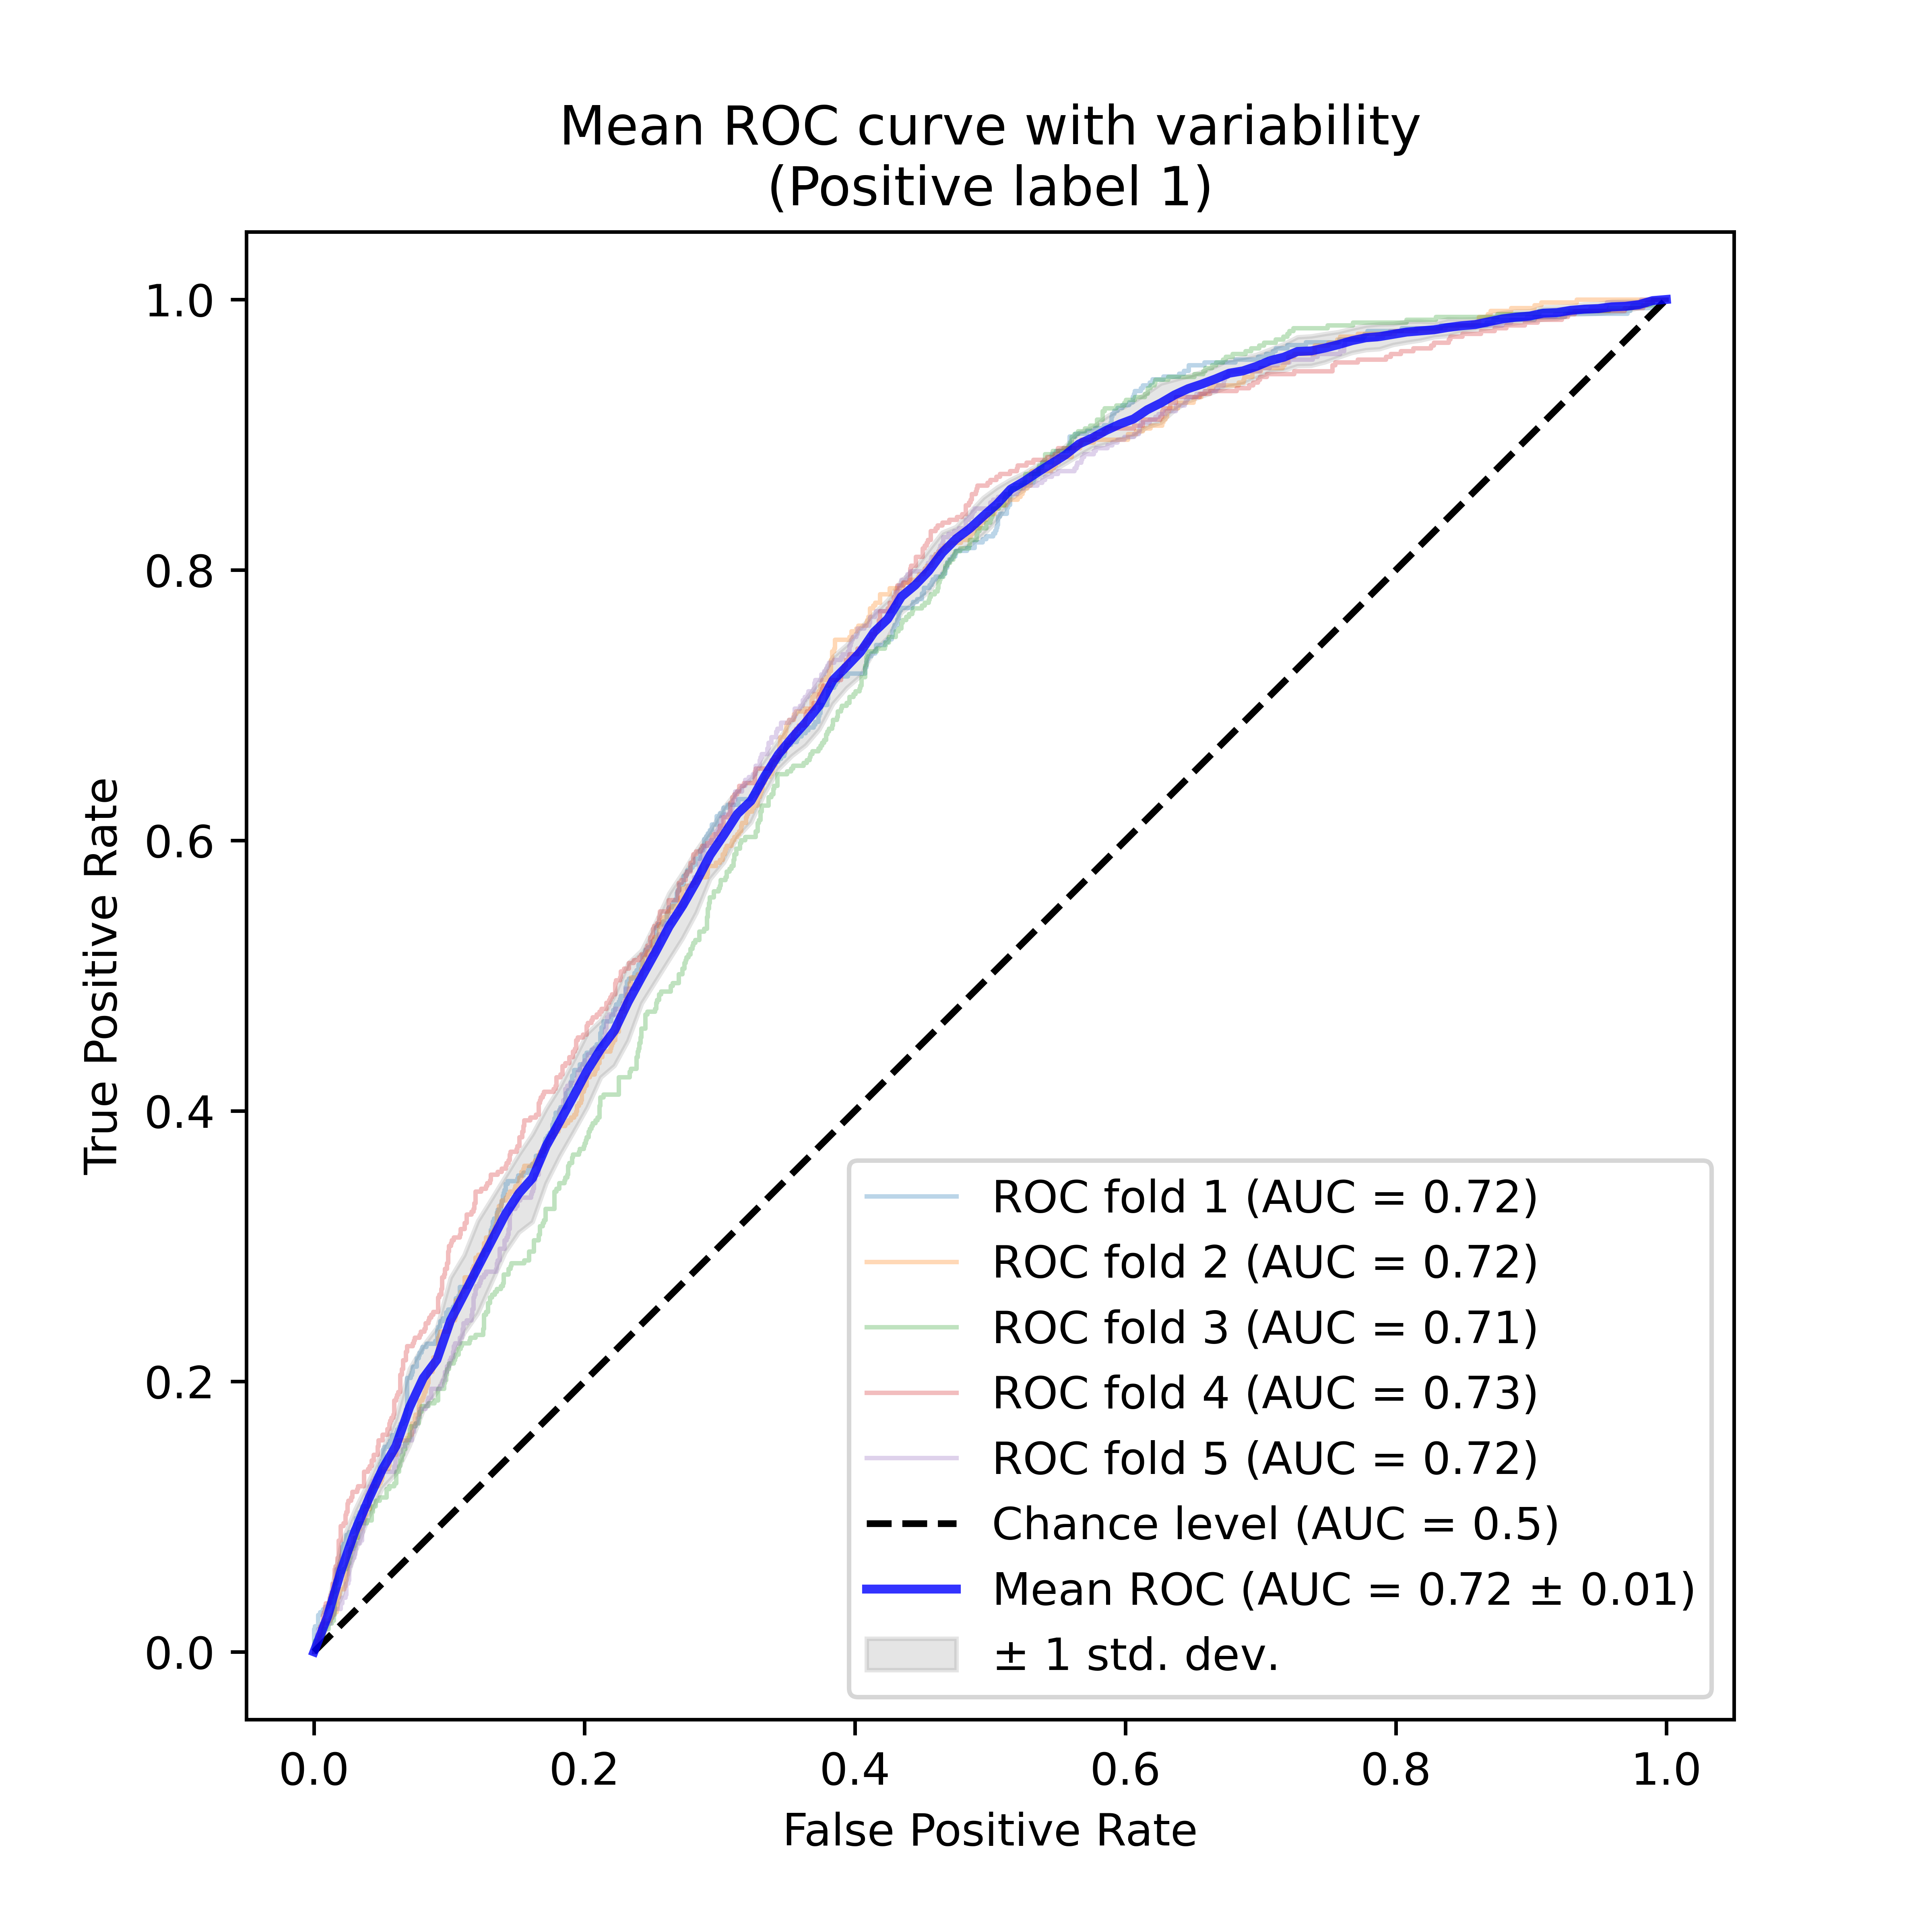
\includegraphics[width=7cm, height=4.8cm]{svm_full_cv_roc.png} }}
    \qquad
    \subfloat[XGB]{{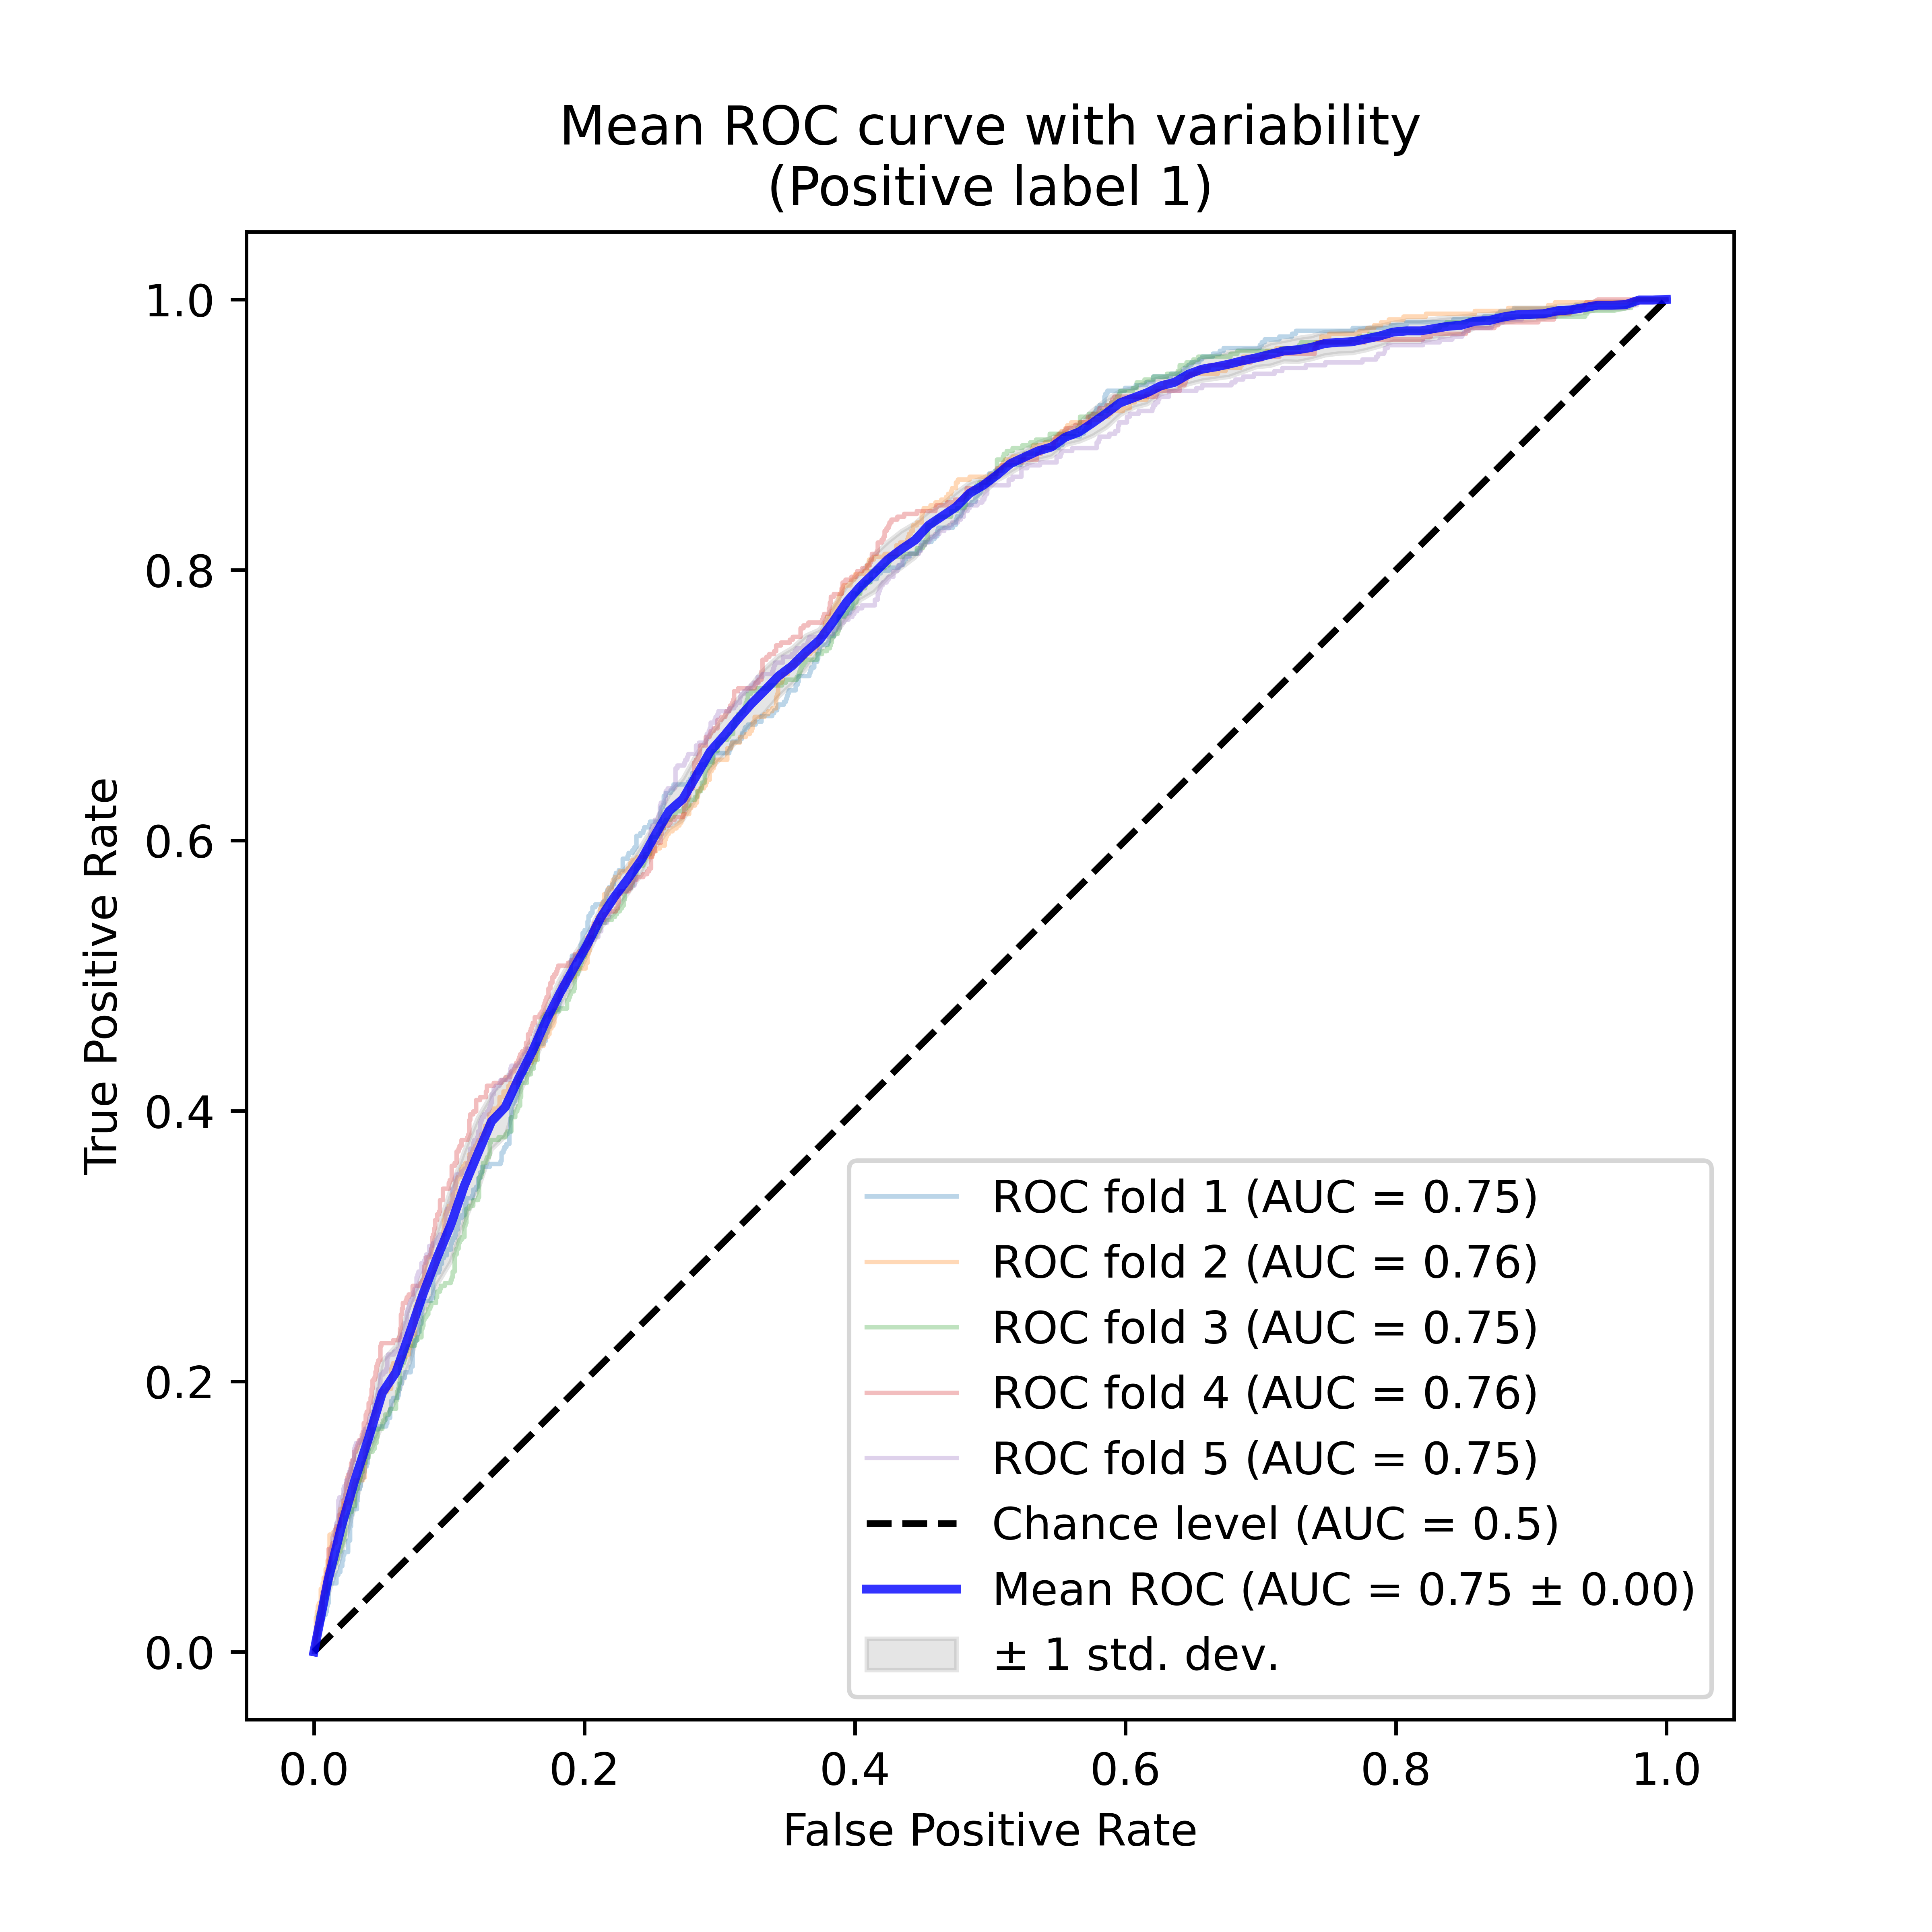
\includegraphics[width=7cm, height=4.8cm]{xgb_full_cv_roc.png} }}
    \caption{Cross validated AUC with full data}
\end{figure}

In both models, RIDAGYR is the most important feature and LBXBCD is the least important feature when we are using the full dataset. 

\begin{figure}[!ht]
    \centering
    \subfloat[SVM]{{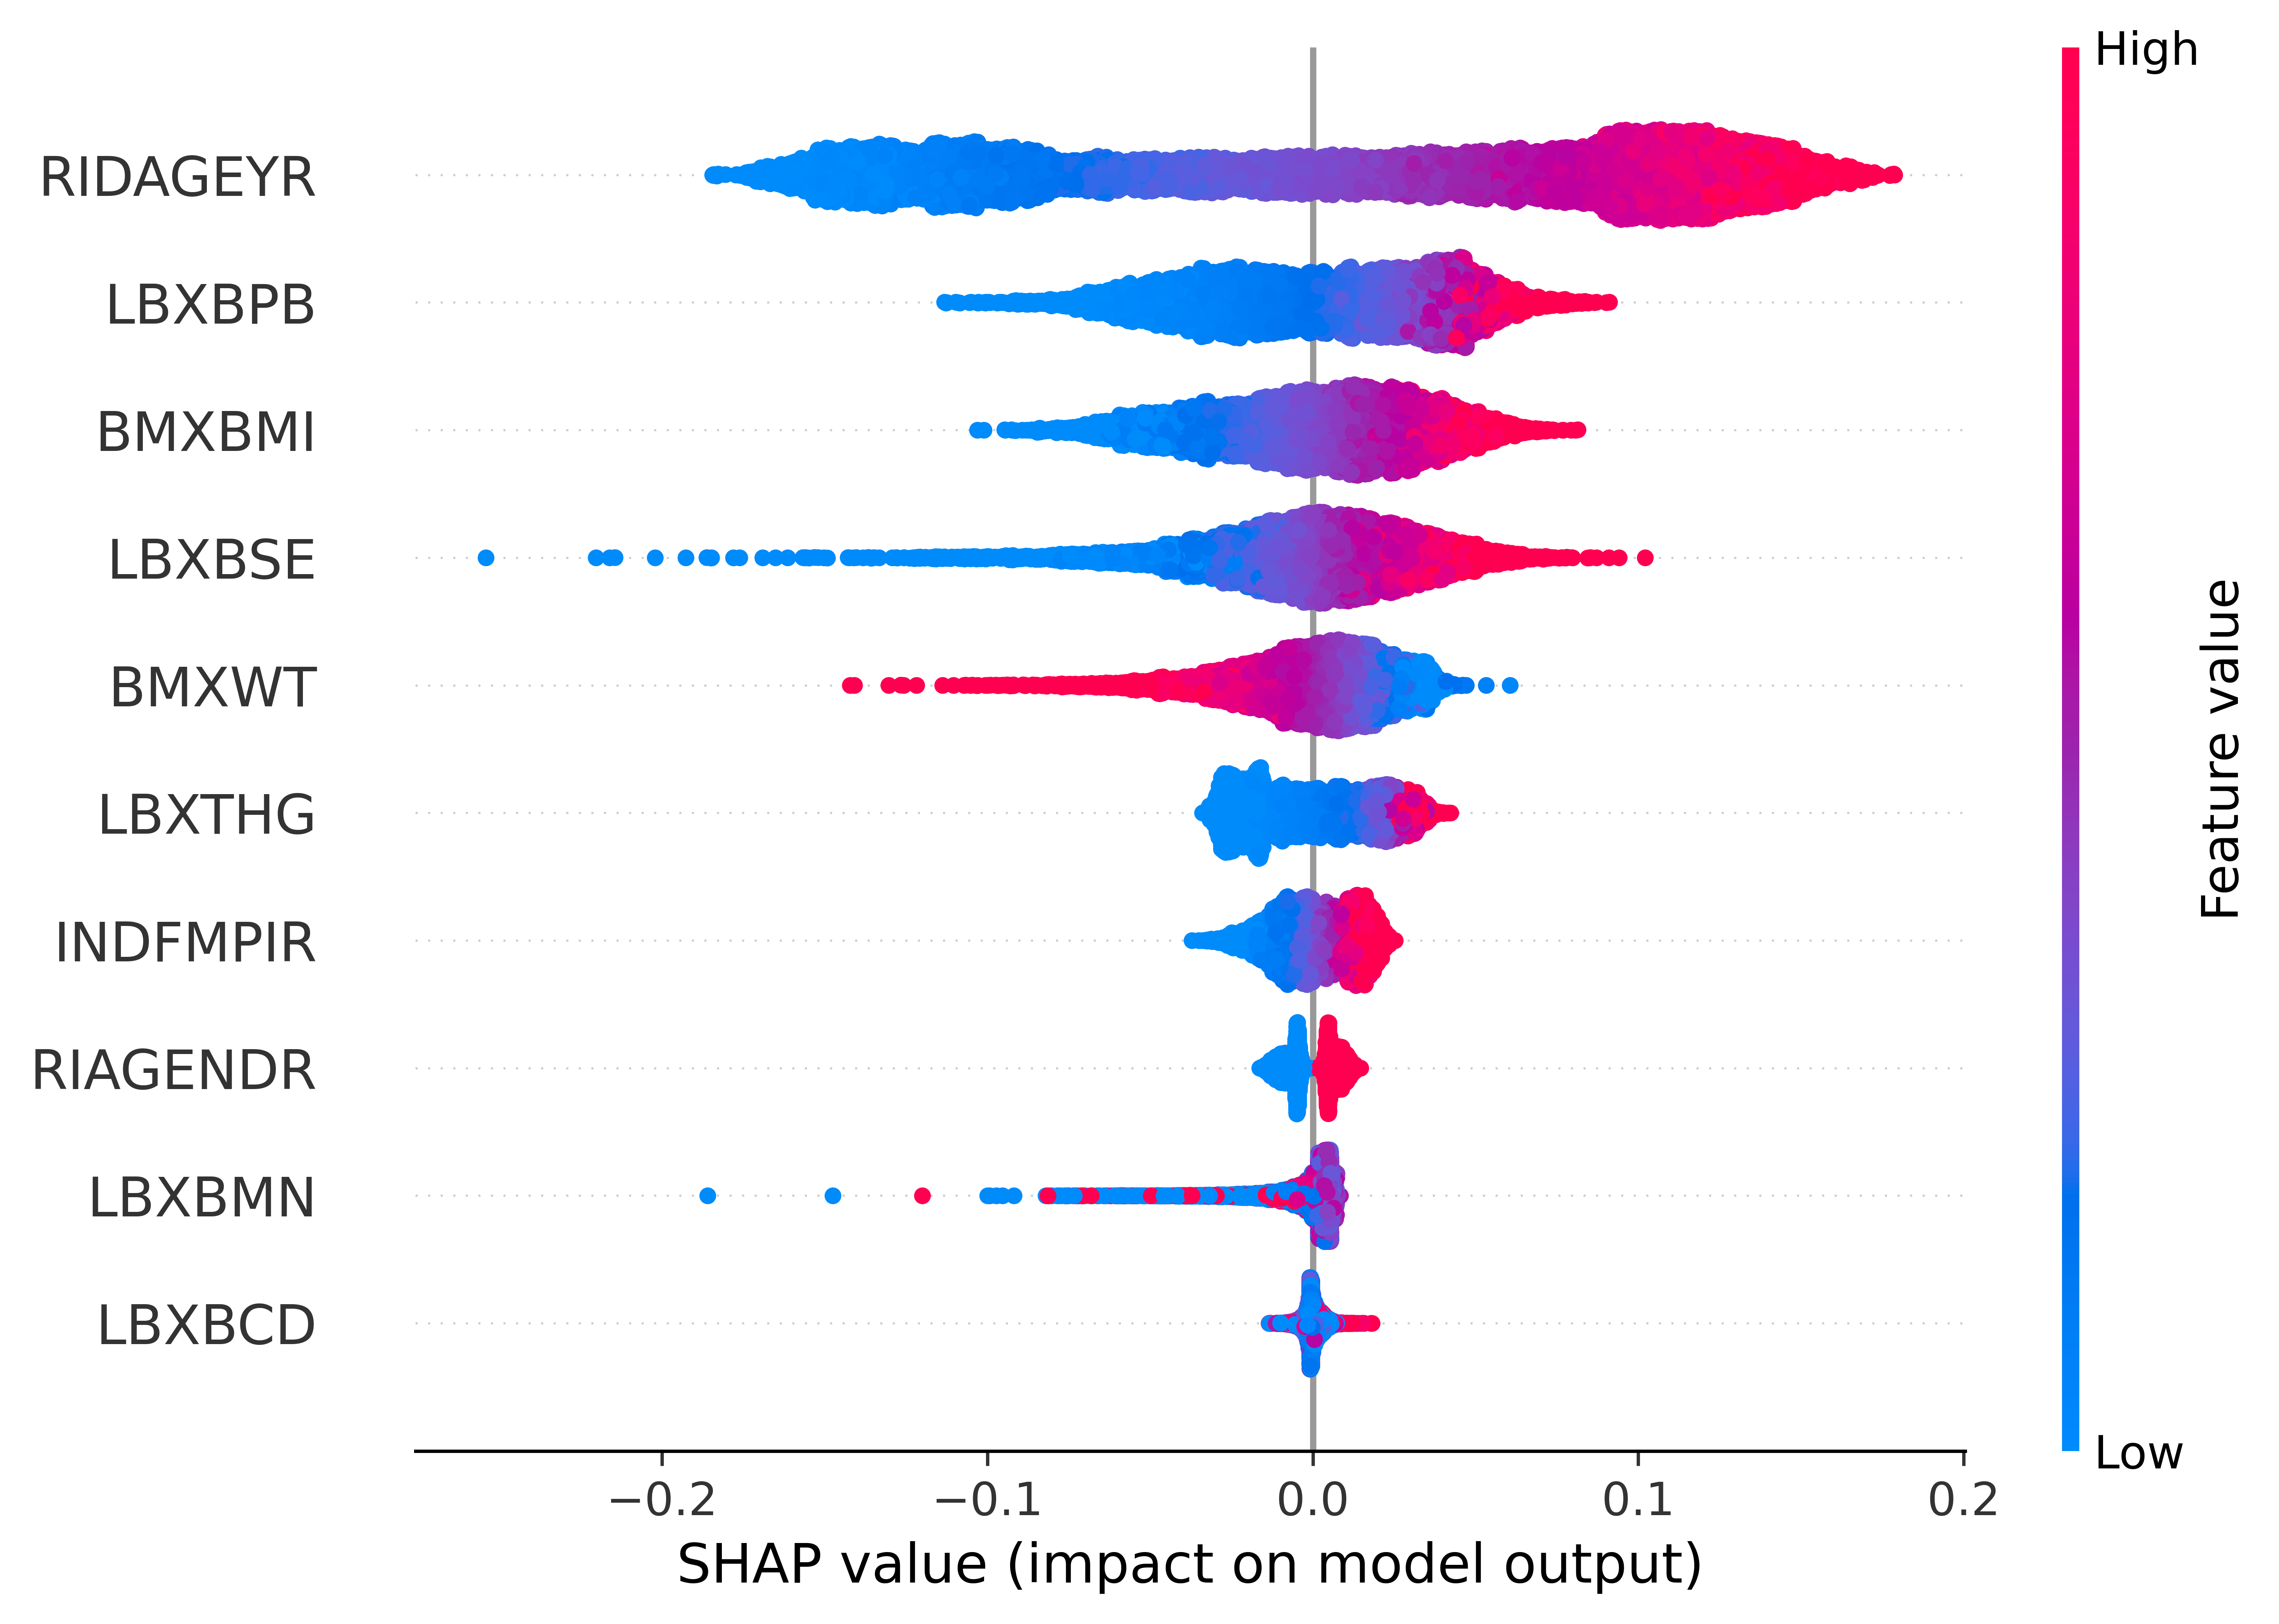
\includegraphics[width=7cm, height=4.8cm]{svm_full_beeswarm.png} }}
    \qquad
    \subfloat[XGB]{{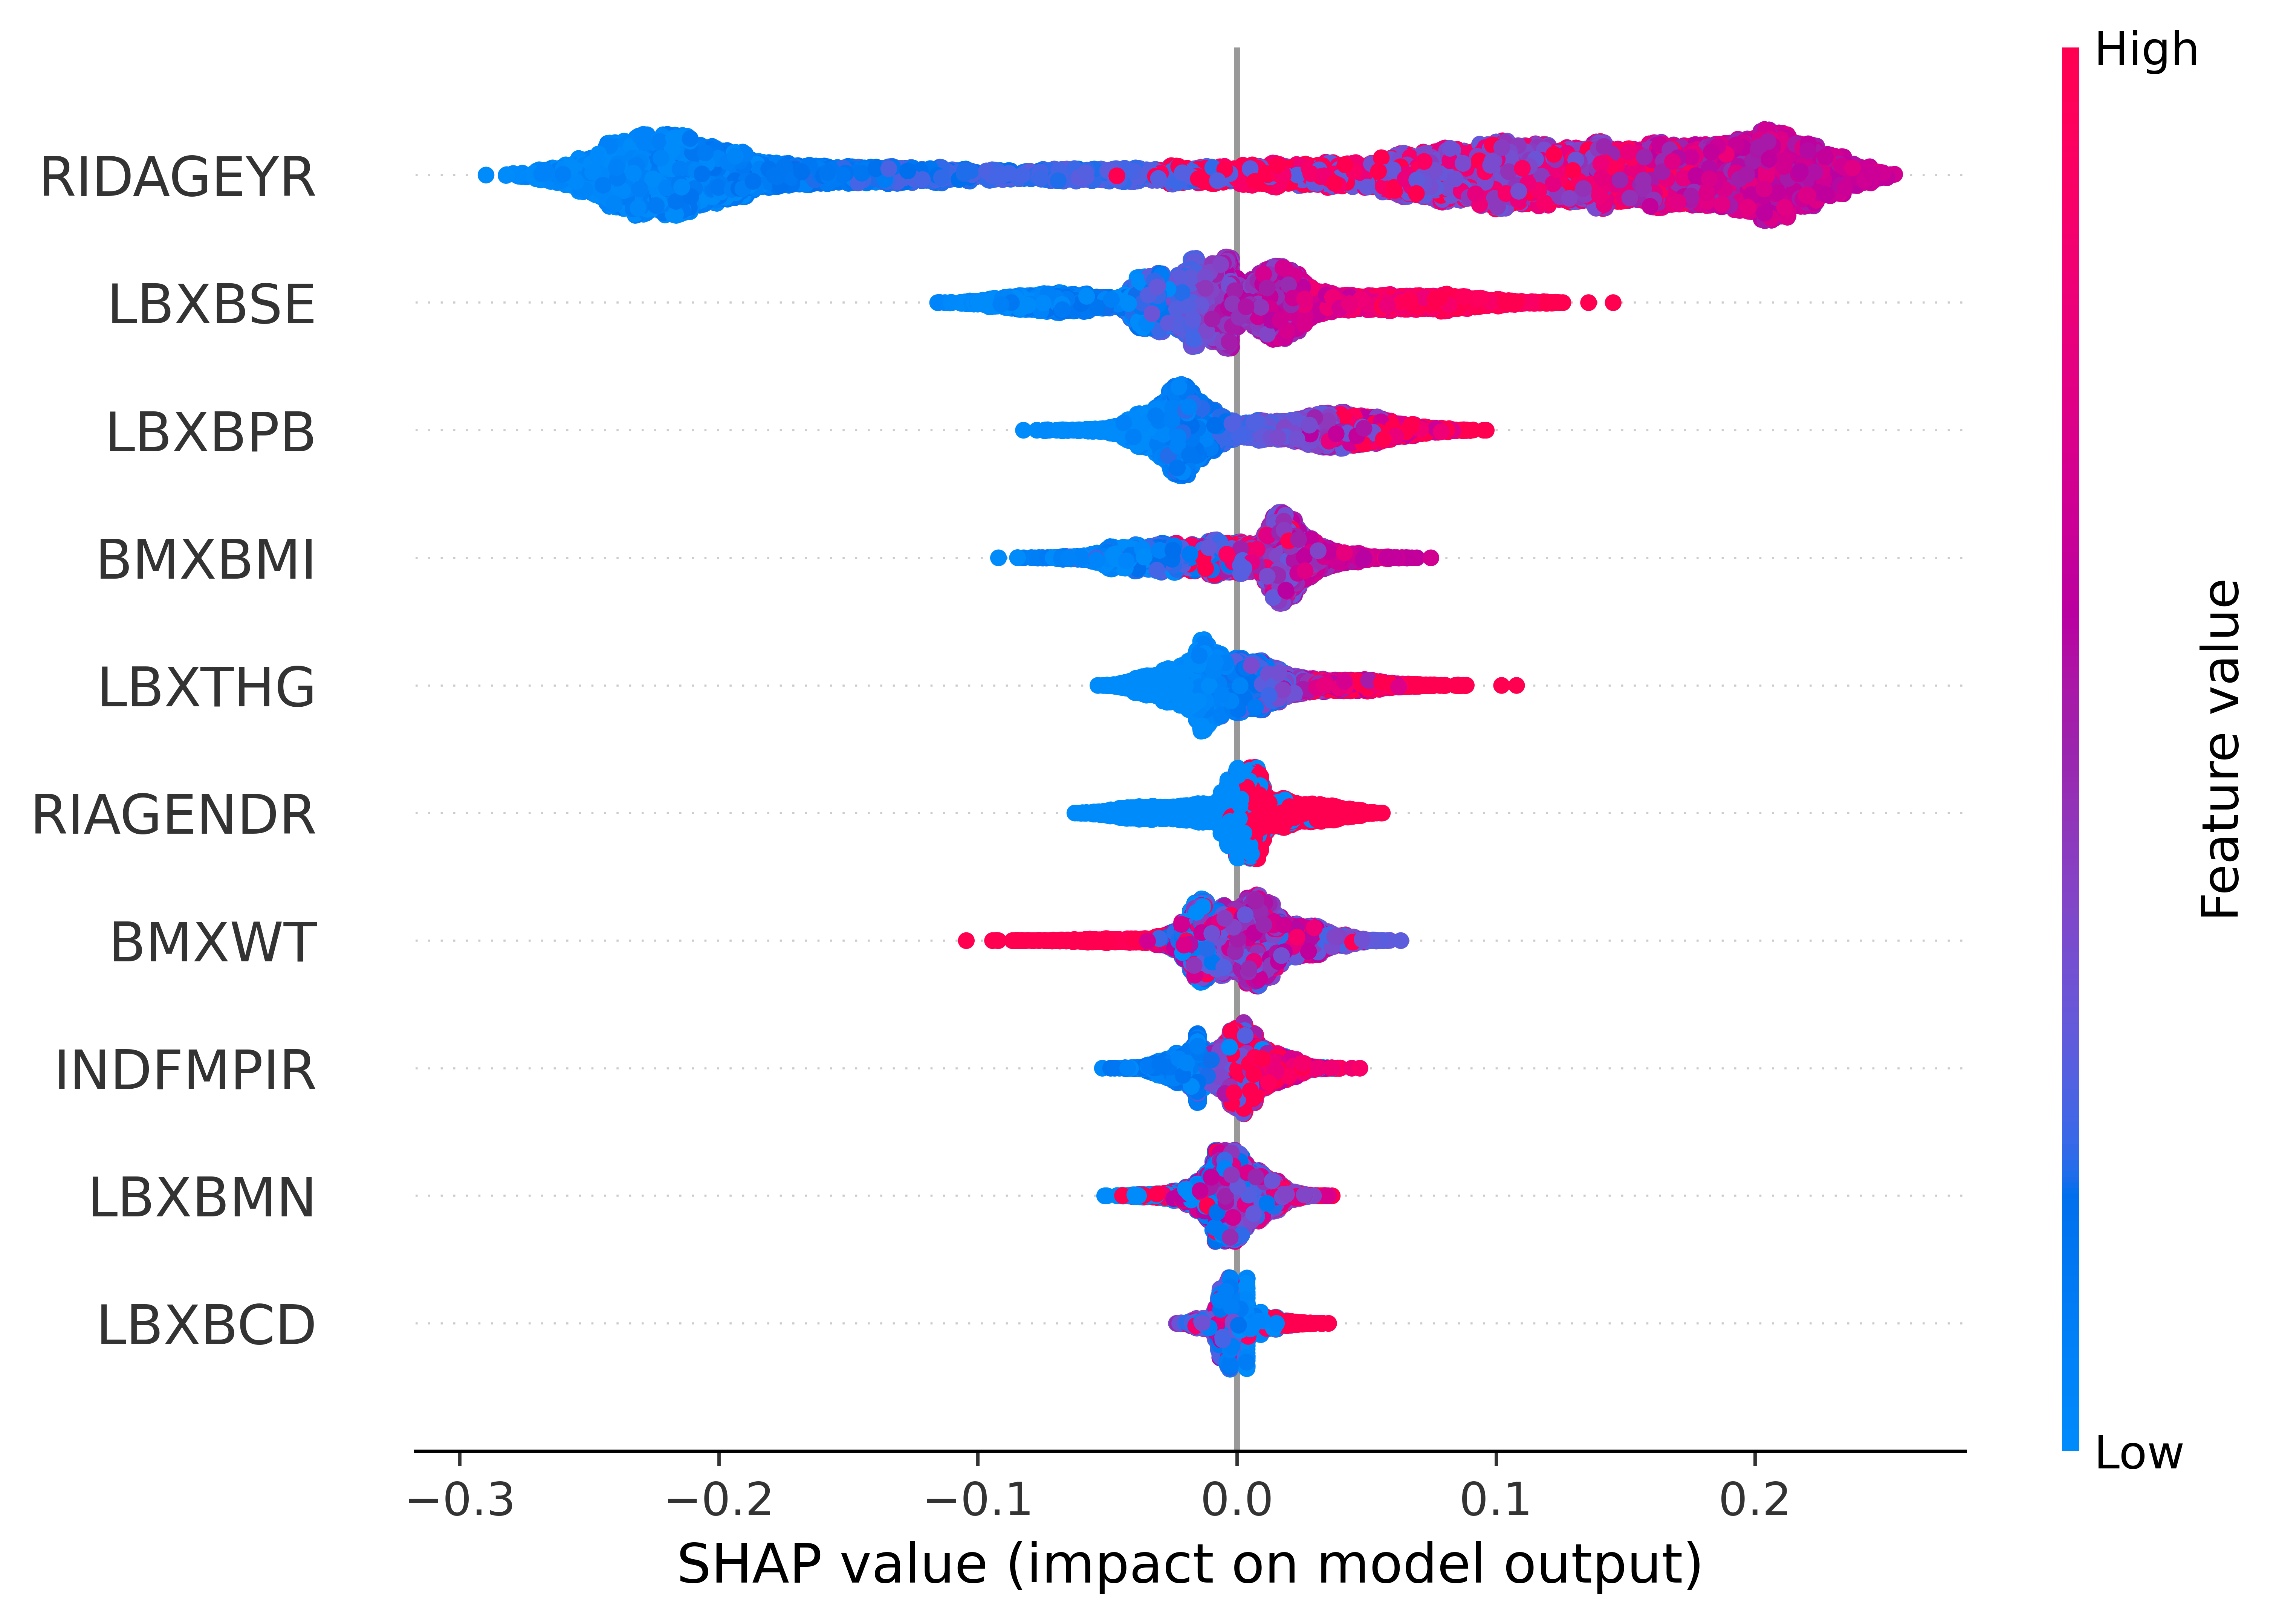
\includegraphics[width=7cm, height=4.8cm]{xgb_full_beeswarm.png} }}
    \caption{Feature importance with full data}
\end{figure}

In the beeswarm plot of feature importance, based on the SHAP values and the corresponding variable values, we can see that older people are more likely to be unhealthy based on SHAP values and corresponding variable values. Additionally, in both models, higher body mass index, family income level, and blood heavy metal concentration tend to correlate to a higher probability of high cholesterol levels. (except for blood manganese concentration, it has mixed effects in both models) However, a counter-intuitive observation is that higher weight is correlated with a lower probability of having high cholesterol levels. (This trend is not obvious in XGB model) Also, in both model, it seems that females are more likely to have high cholesterol levels, which does not have a clear scientific explanation.

For SVM model, the F1 value is 0.512, the balanced accuracy is 0.674, and the ROC-AUC value is 0.719. For XGBoost model, the F1 value is 0.529, the balanced accuracy is 0.69, and the ROC-AUC value is 0.754.

\subsection{Subsets}

Based on the result of models using the full dataset, we know that the most important feature is RIDAGYR(age). In this case, we divided the data into three subsets based on the age of the participant:

\begin{itemize}
    \item \texttt{Young group}: Participants with age range 0 to 30.
    \item \texttt{Middle group}:  Participants with age range 30 to 60.
    \item \texttt{Old group}: Participants with age range 60 to 90.
\end{itemize}

Since grouping may cause deterioration in model performance, we only use the better model structure from the previous problem.

\subsubsection{Young Group}

For the SVM model, the AUC values for each fold ranged from 0.66 to 0.74, with an average AUC of 0.71. For XGB model, the AUC values for each fold ranged from 0.65 to 0.74, with a mean AUC of 0.71.

\begin{figure}[!ht]
    \centering
    \subfloat[SVM]{{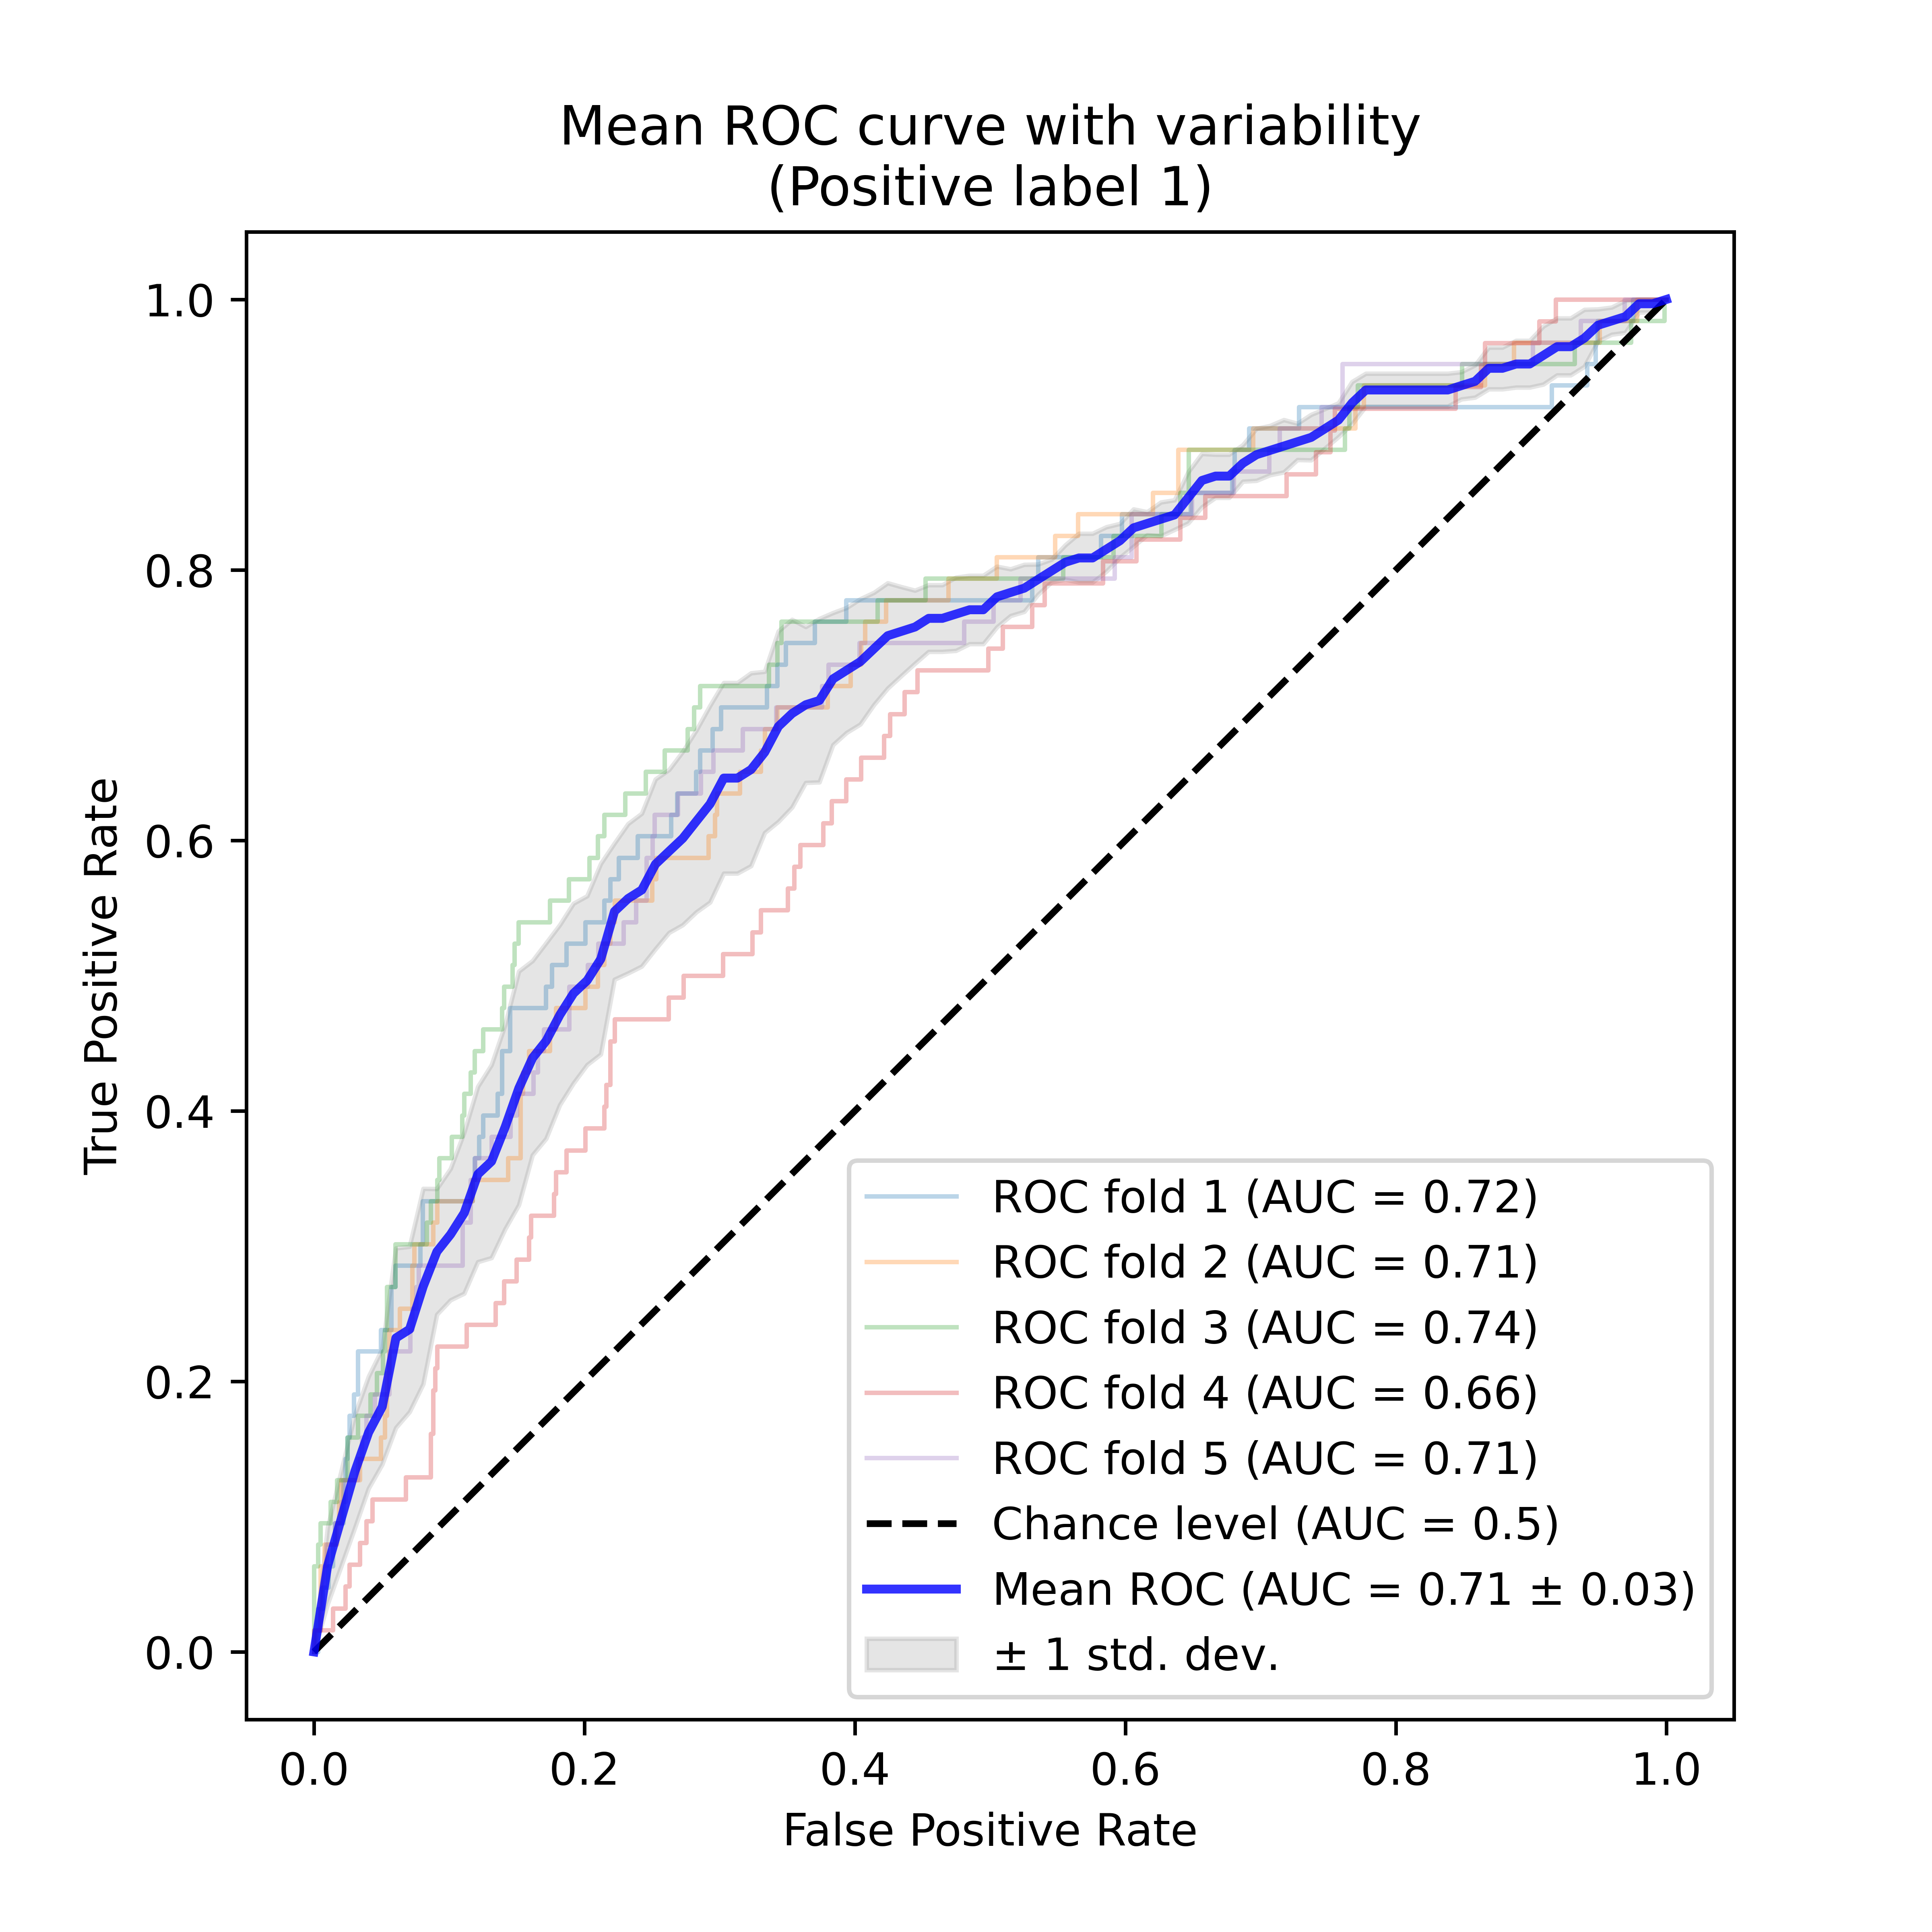
\includegraphics[width=7cm, height=4.8cm]{svm_young_cv_roc.png} }}
    \qquad
    \subfloat[XGB]{{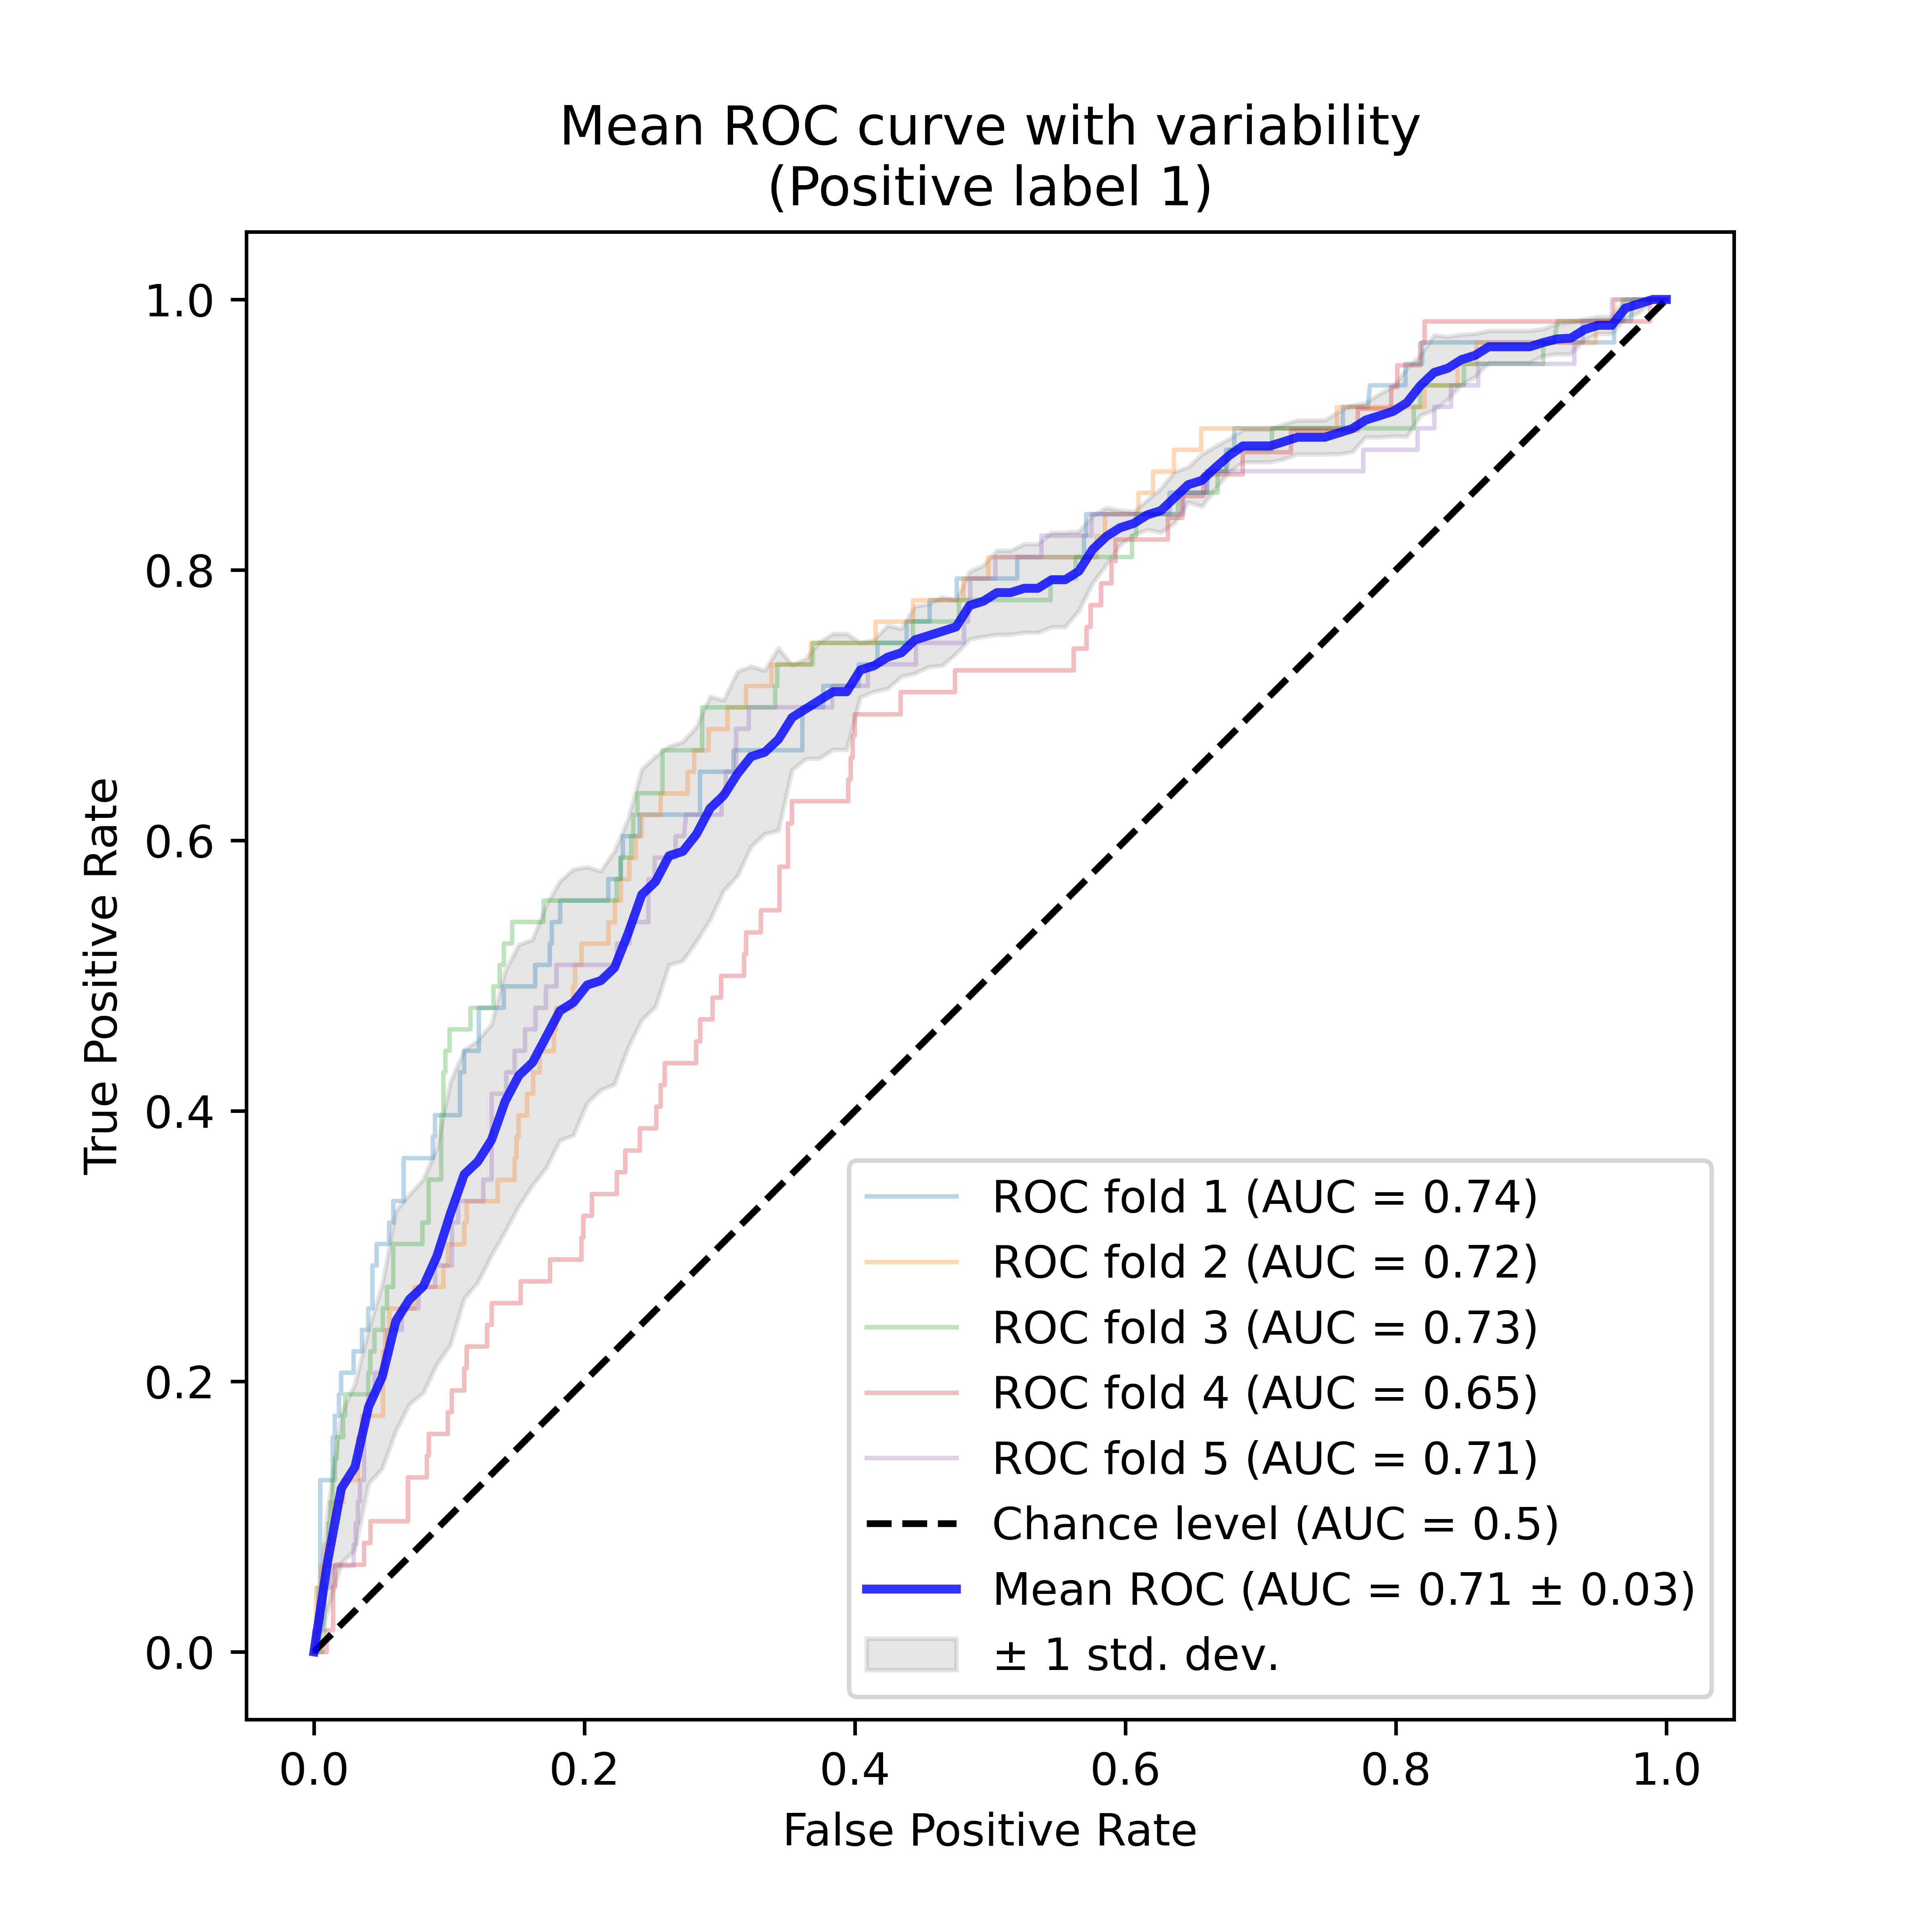
\includegraphics[width=7cm, height=4.8cm]{xgb_young_cv_roc.png} }}
    \caption{Cross validated AUC for young group}
\end{figure}

When we only use the young group of the entire dataset, RIDAGYR remains the most important feature of both models. However, for the least important feature, LBXBCD is the least important feature in the SVM model, but when we use the XGB model, RIAGENDR is the new least important feature. Most of the trends are the same as the full data, but there are a few differences. In this case, the blood magnesium concentration has displayed a clear negative correlation with the probability of having high cholesterol levels. Also, blood cadmium concentration also has displayed a negative correlation with the probability of having high cholesterol levels. Additionally, it seems that young males are more likely to have high cholesterol levels than young females, which is opposite to the effect observed by using the full data. Lastly, the XGB model has displayed a positive correlation between body weight and the probability of having high cholesterol levels. (differs from SVM model)

\begin{figure}[!ht]
    \centering
    \subfloat[SVM]{{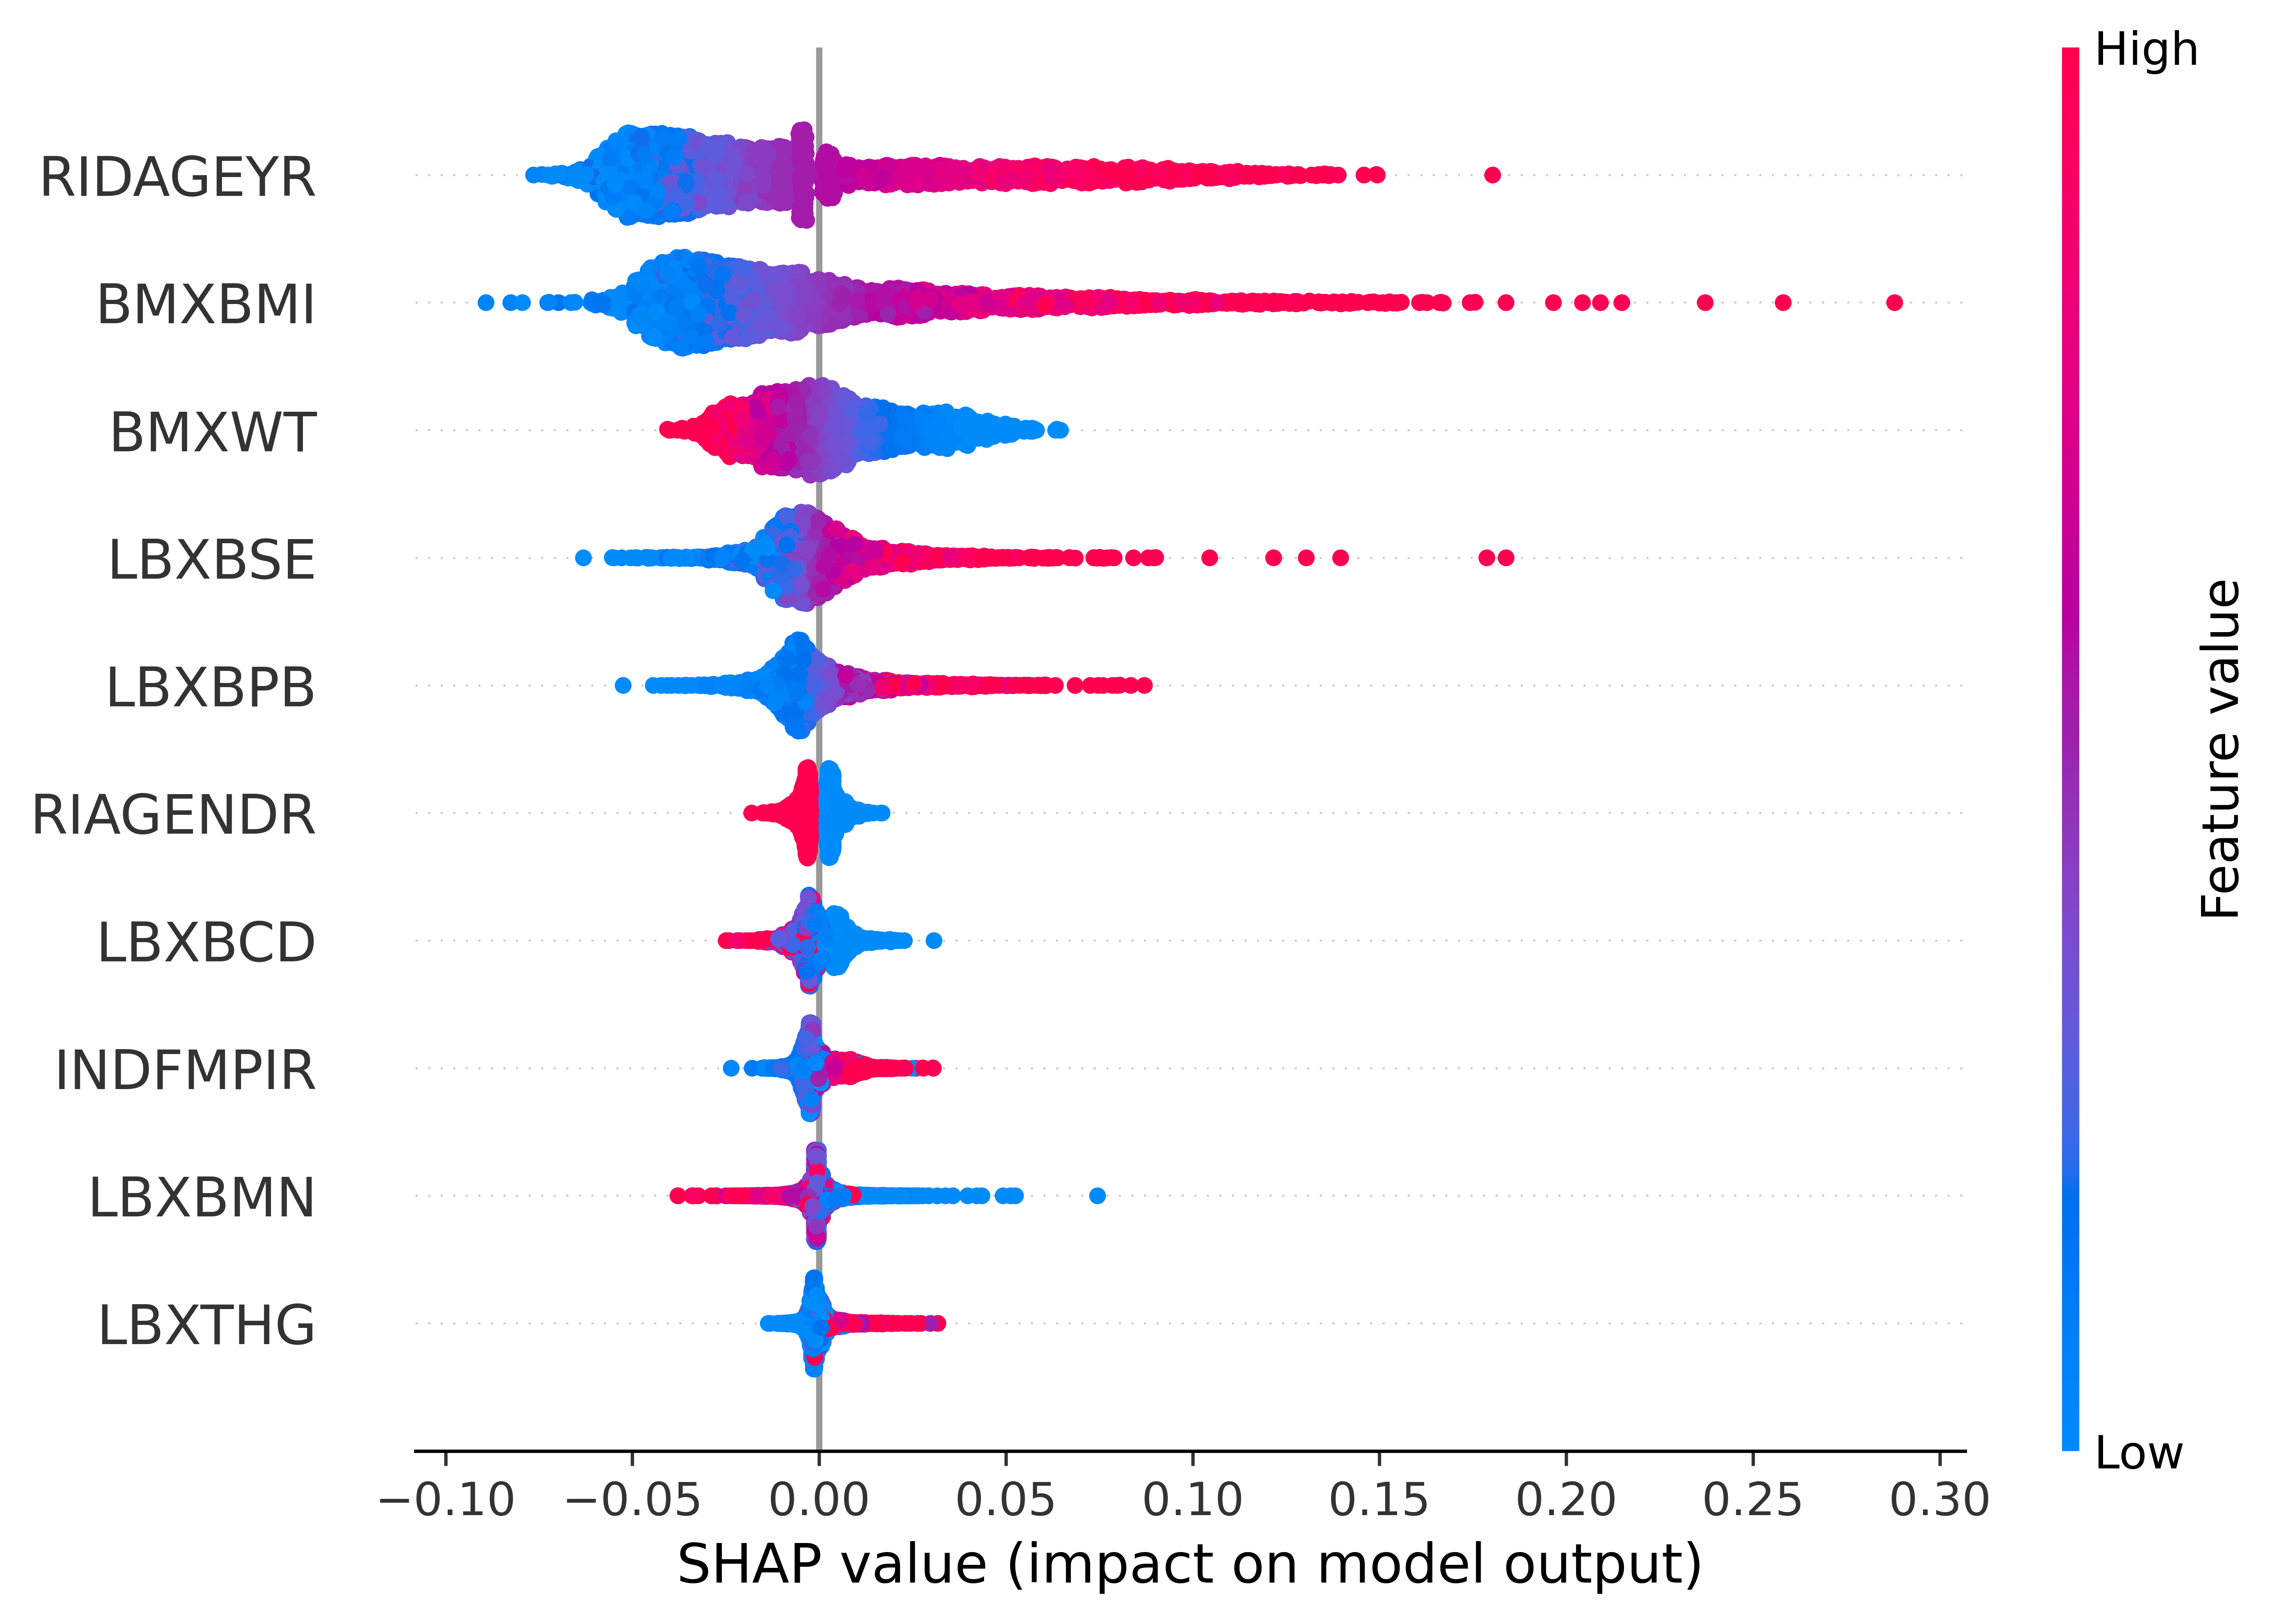
\includegraphics[width=7cm, height=4.8cm]{svm_young_beeswarm.png} }}
    \qquad
    \subfloat[XGB]{{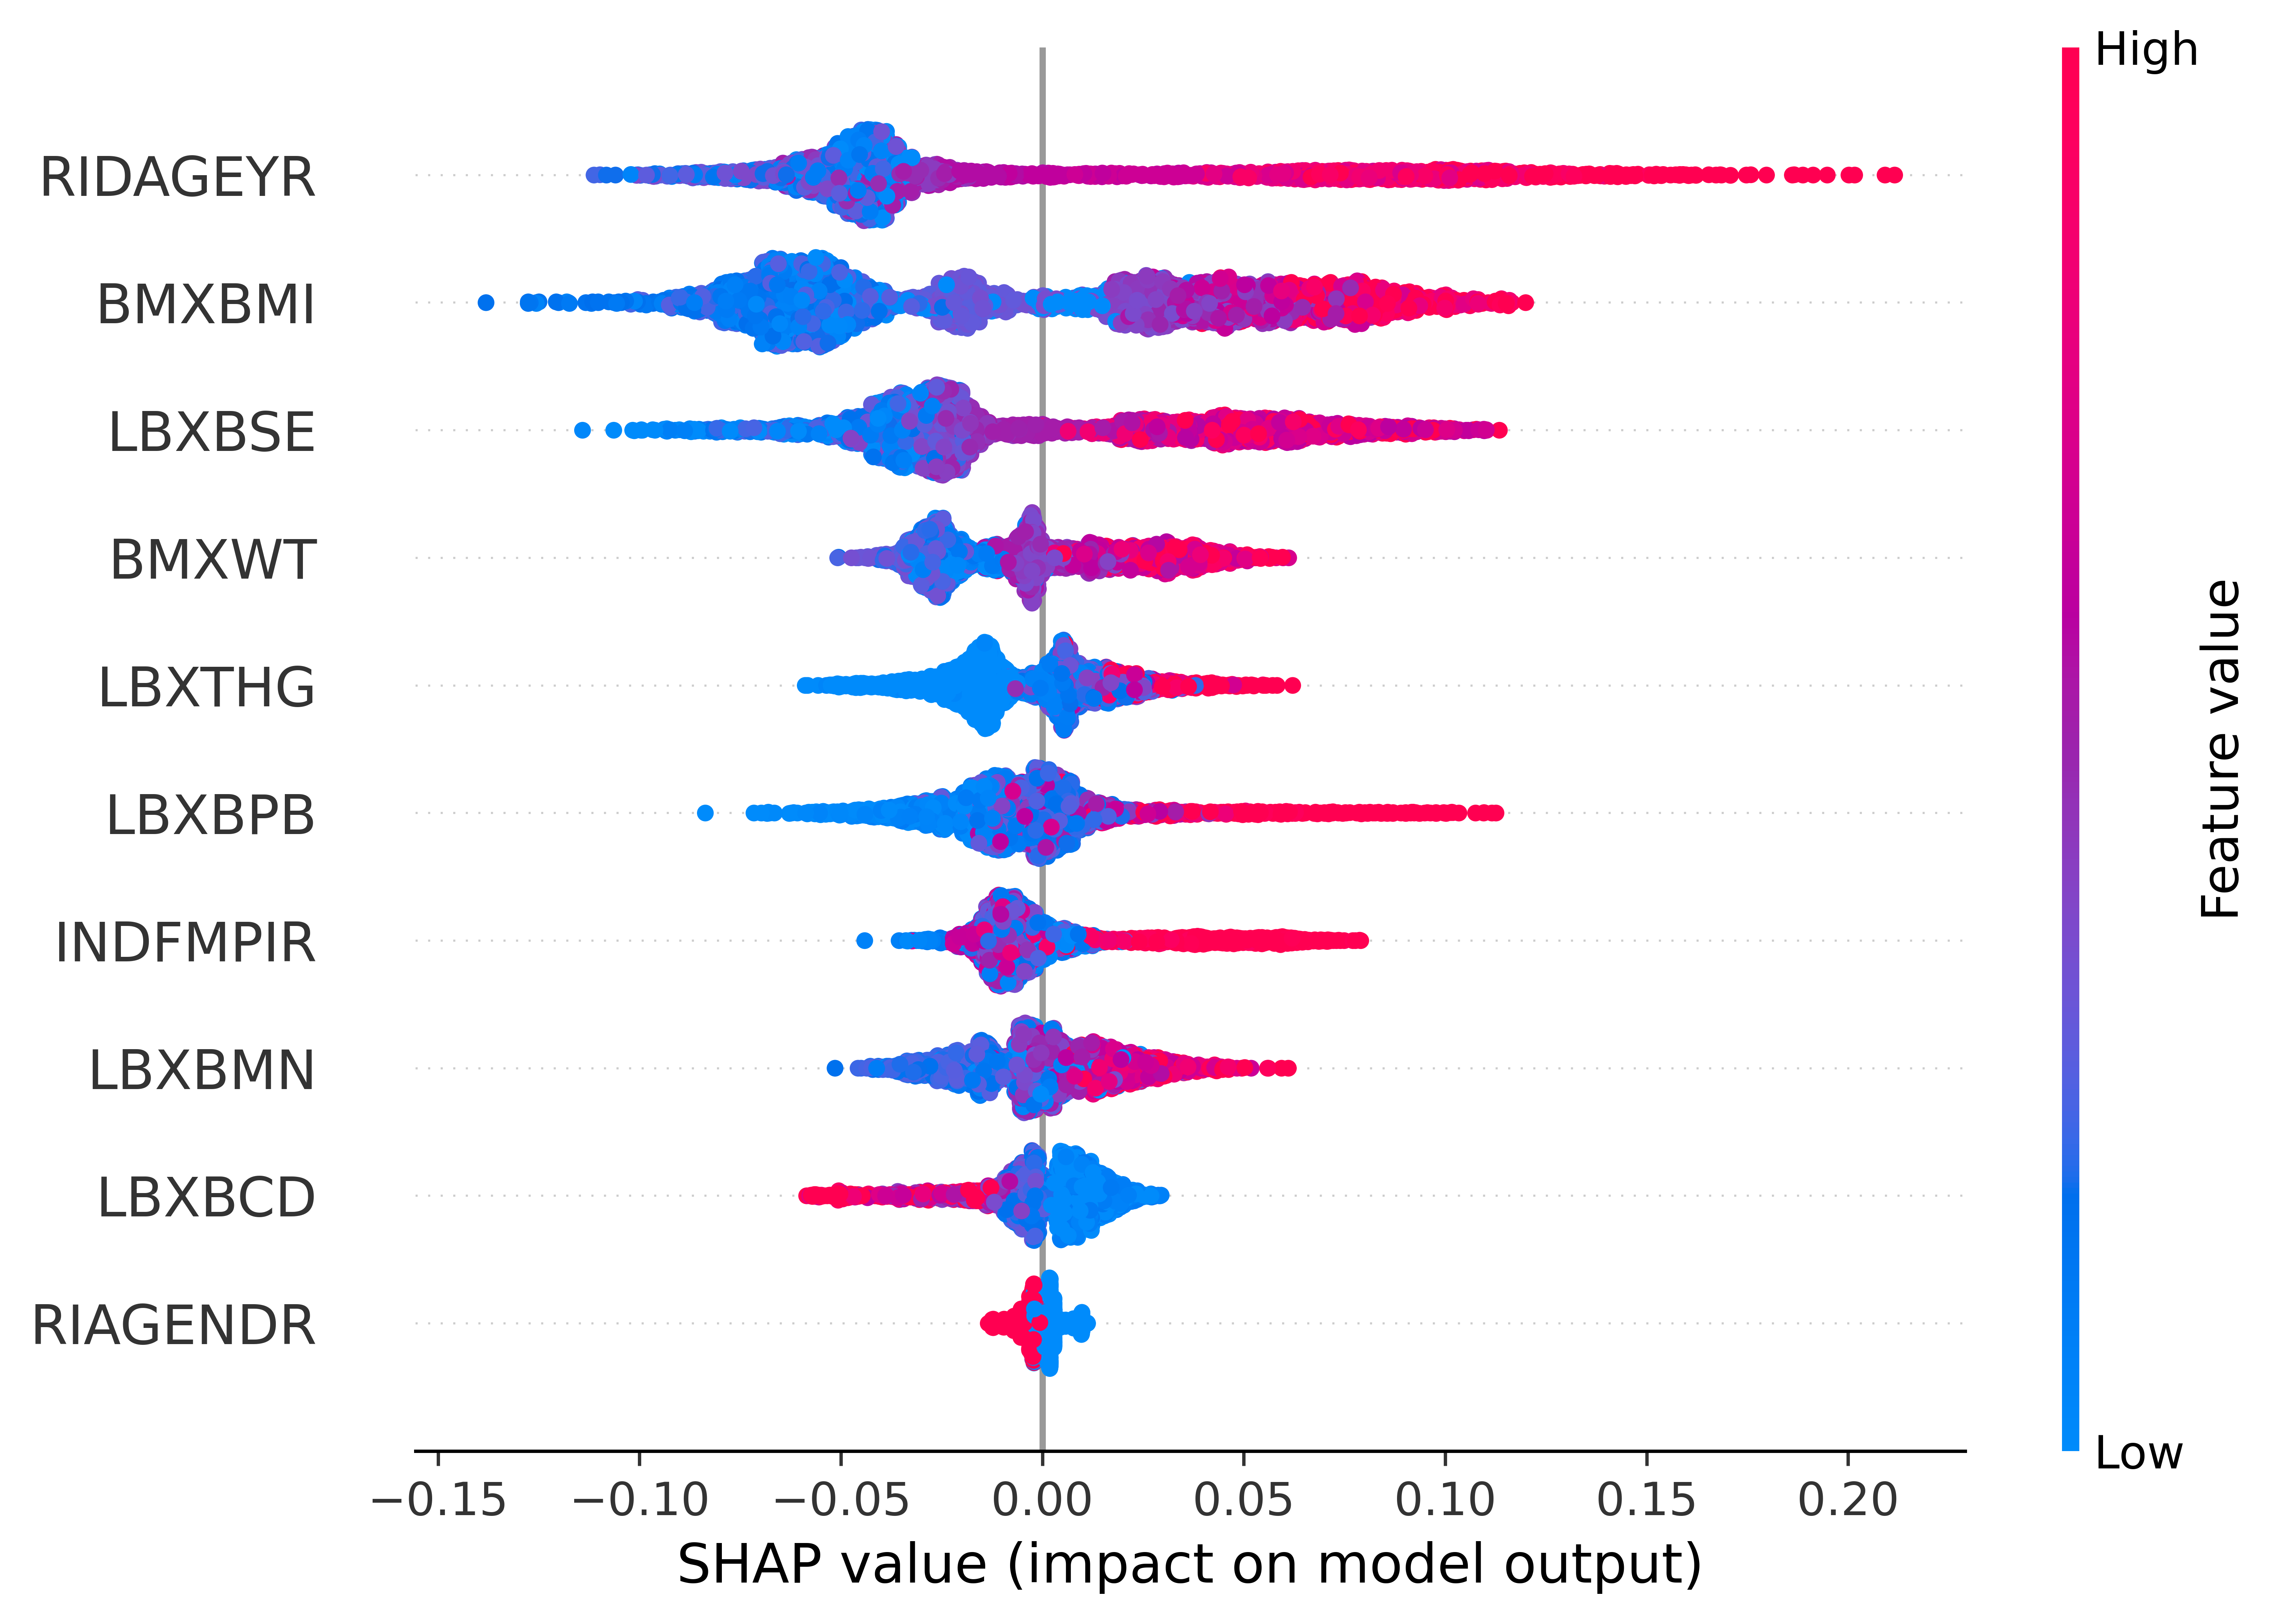
\includegraphics[width=7cm, height=4.8cm]{xgb_young_beeswarm.png} }}
    \caption{Feature importance for young group}
\end{figure}

When we are using the young group subset, for SVM model, the F1 value is 0.271, the balanced accuracy is 0.666, and the ROC-AUC value is 0.709. For XGBoost model, the F1 value is 0.243, the balanced accuracy is 0.58, and the ROC-AUC value is 0.71.

\subsubsection{Middle Group}

For the SVM model, the AUC values for each fold ranged from 0.60 to 0.65, with an average AUC of 0.62. For XGB model, the AUC values for each fold ranged from 0.61 to 0.64, with a mean AUC of 0.63.

\begin{figure}[!ht]
    \centering
    \subfloat[SVM]{{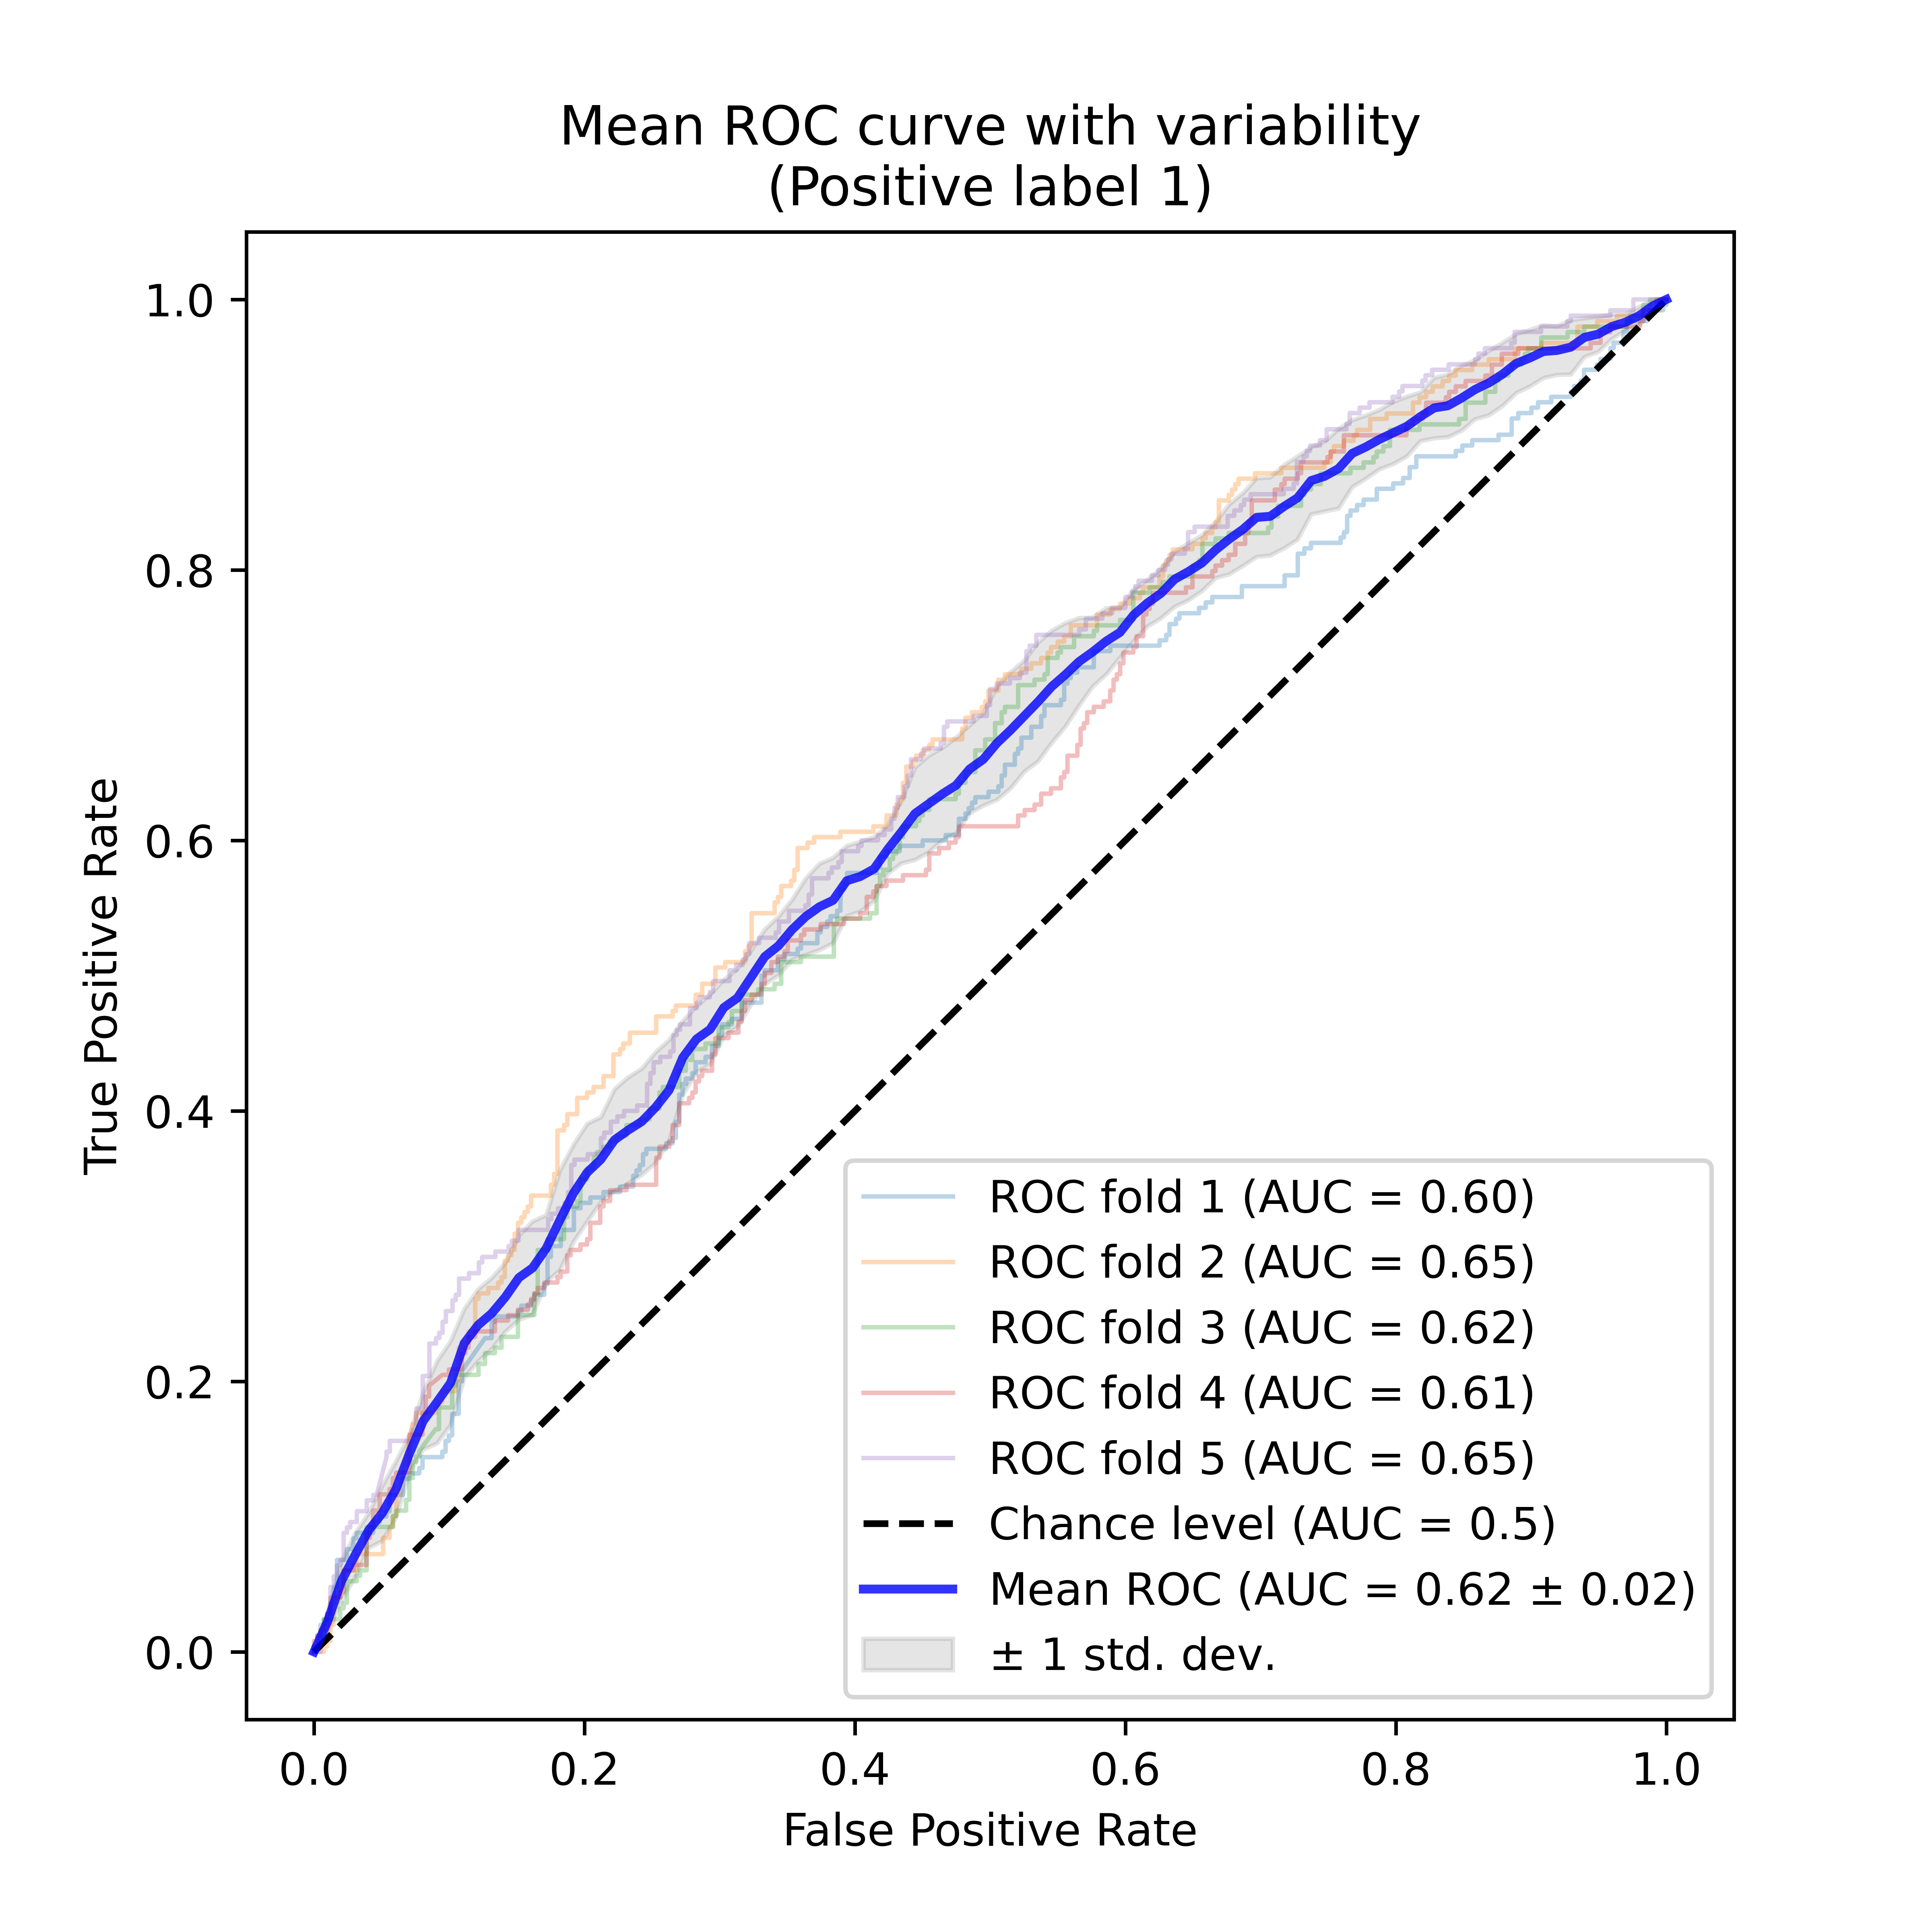
\includegraphics[width=7cm, height=4.8cm]{svm_mid_cv_roc.png} }}
    \qquad
    \subfloat[XGB]{{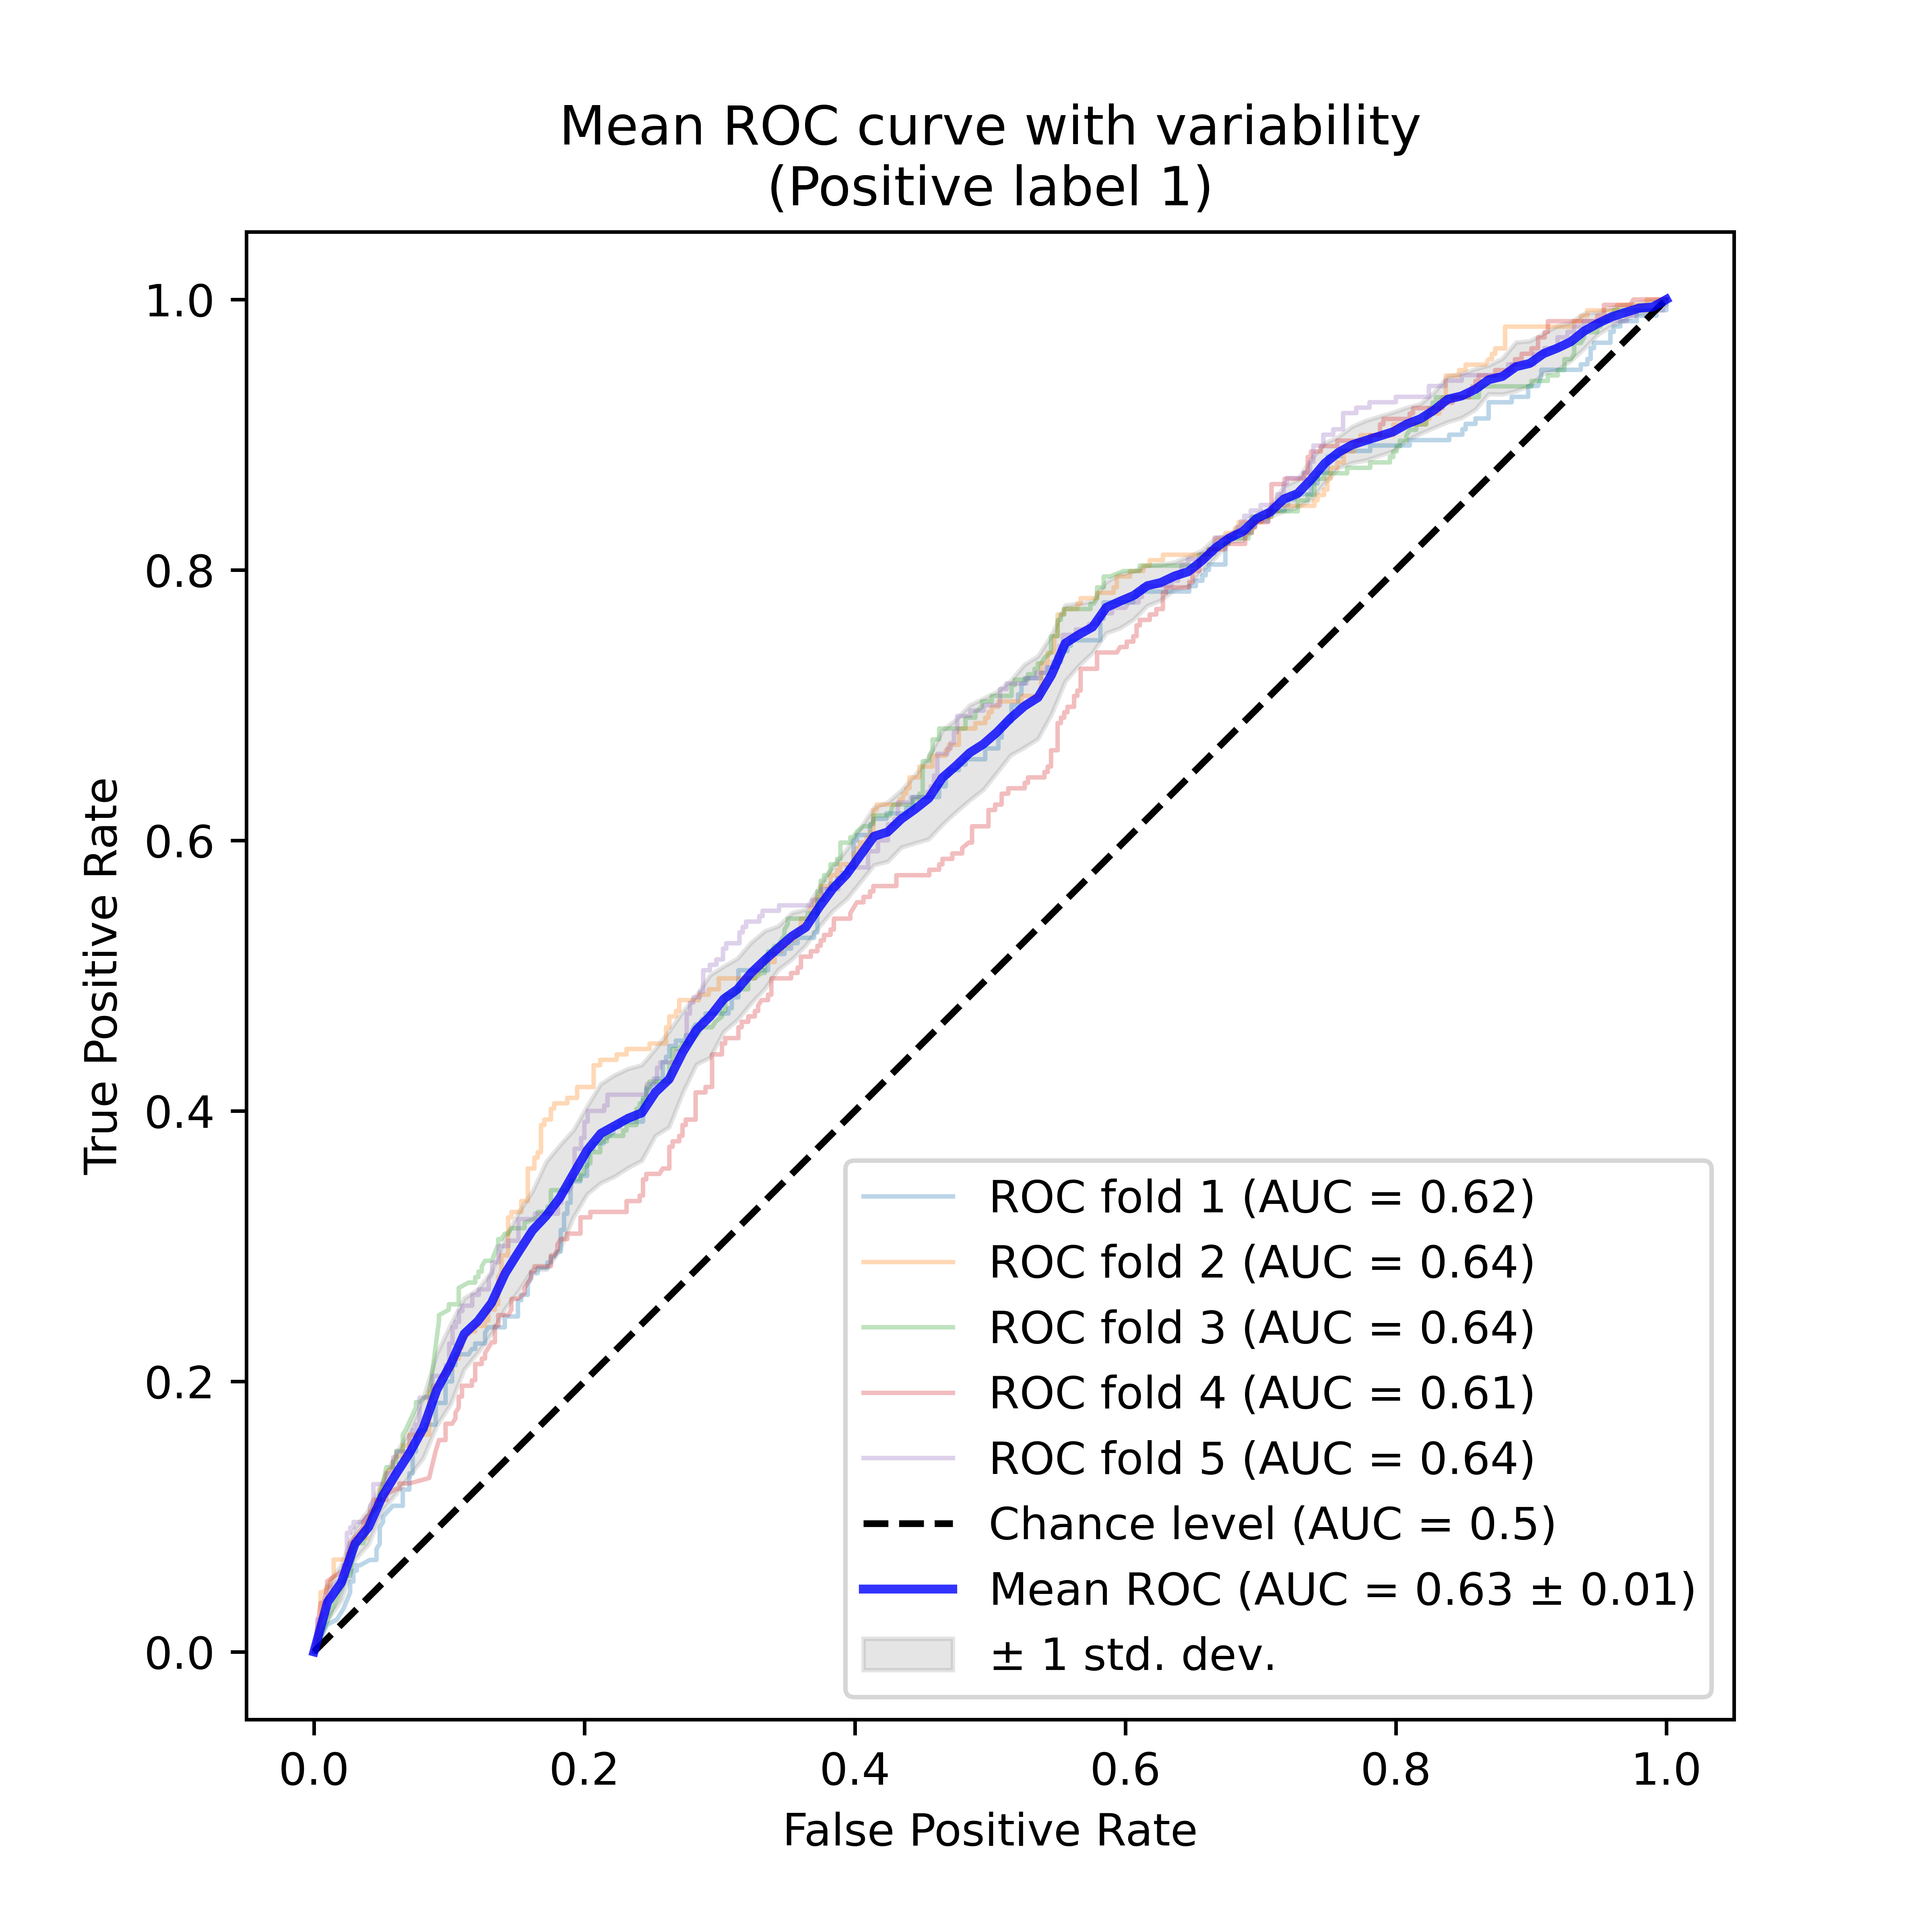
\includegraphics[width=7cm, height=4.8cm]{xgb_mid_cv_roc.png} }}
    \caption{Cross validated AUC for mid group}
\end{figure}

When we only use the middle group of the entire dataset, RIDAGYR remains the most important feature of both models. However, for the least important feature, LBXBCD is the least important feature in the SVM model, but when we use the XGB model, INDFMPIR is the new least important feature. In this case, there are a few changes from the young group models worth noting. The XGB model has displayed a negative correlation between body weight and the probability of having high cholesterol levels. Also, the XGB model seems to display that family income have mixed effects, lower family income can have both positive and negative effect on the probability of having high cholesterol levels.

\begin{figure}[!ht]
    \centering
    \subfloat[SVM]{{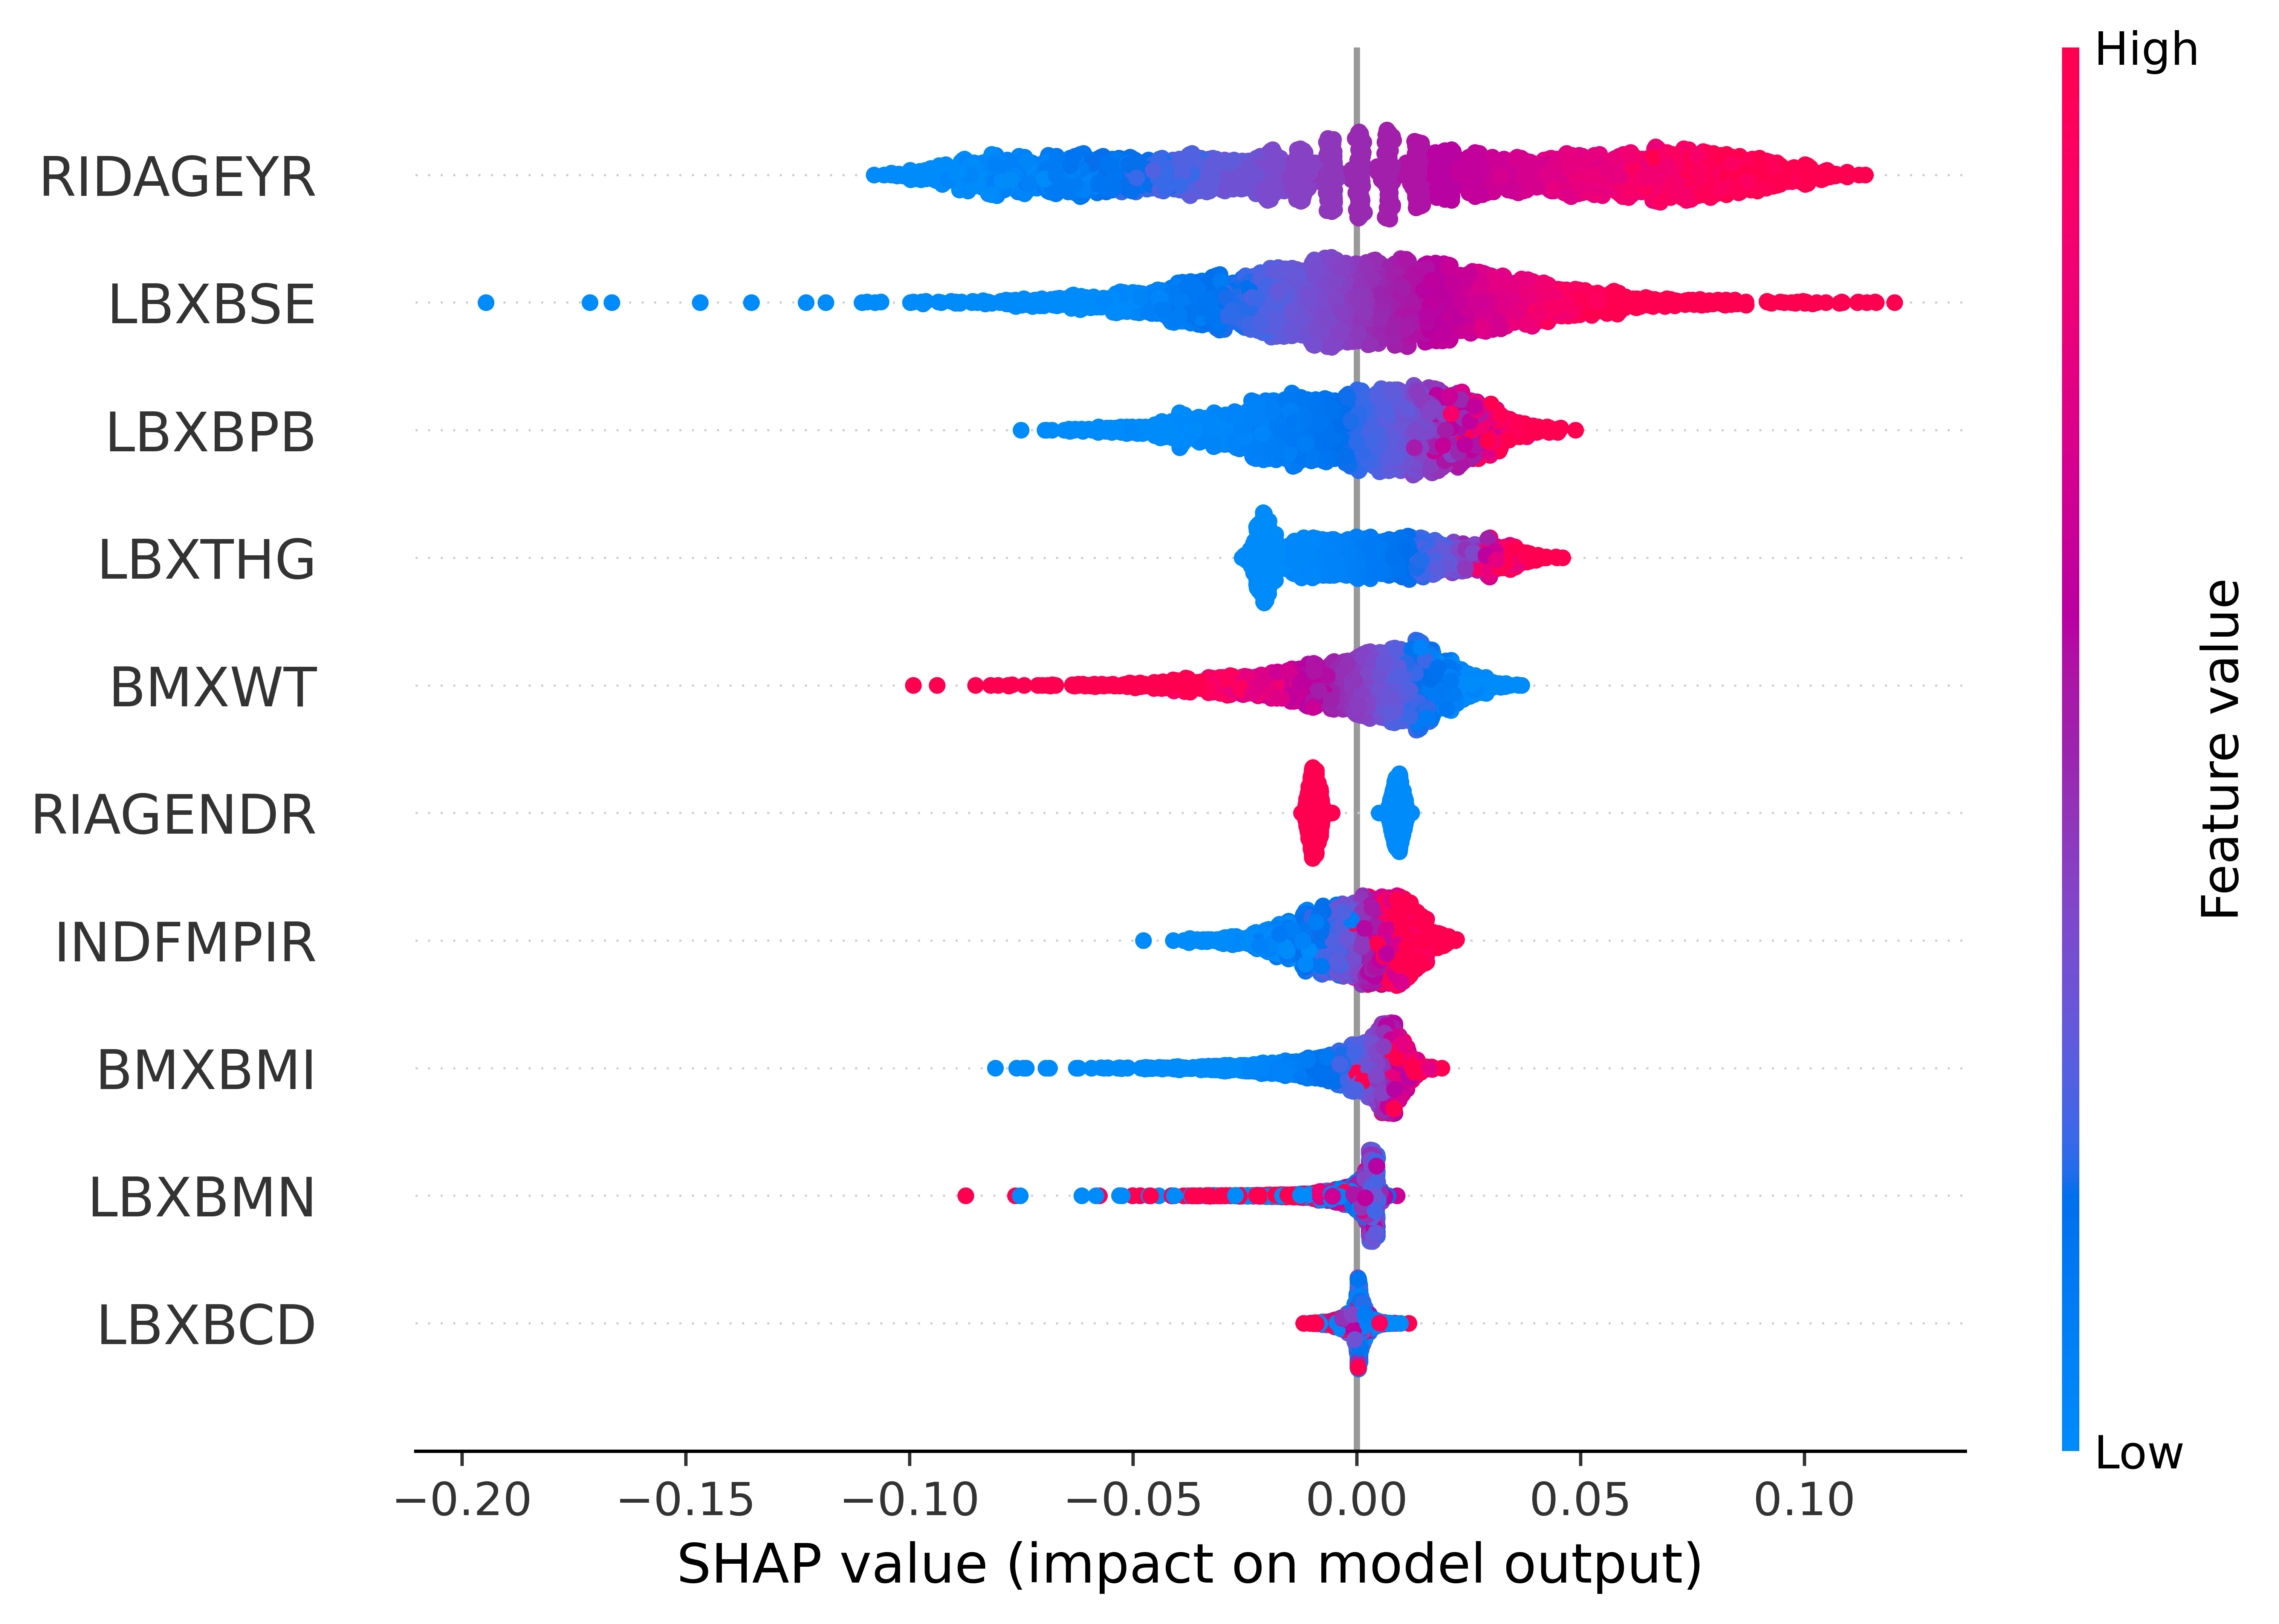
\includegraphics[width=7cm, height=4.8cm]{svm_mid_beeswarm.png} }}
    \qquad
    \subfloat[XGB]{{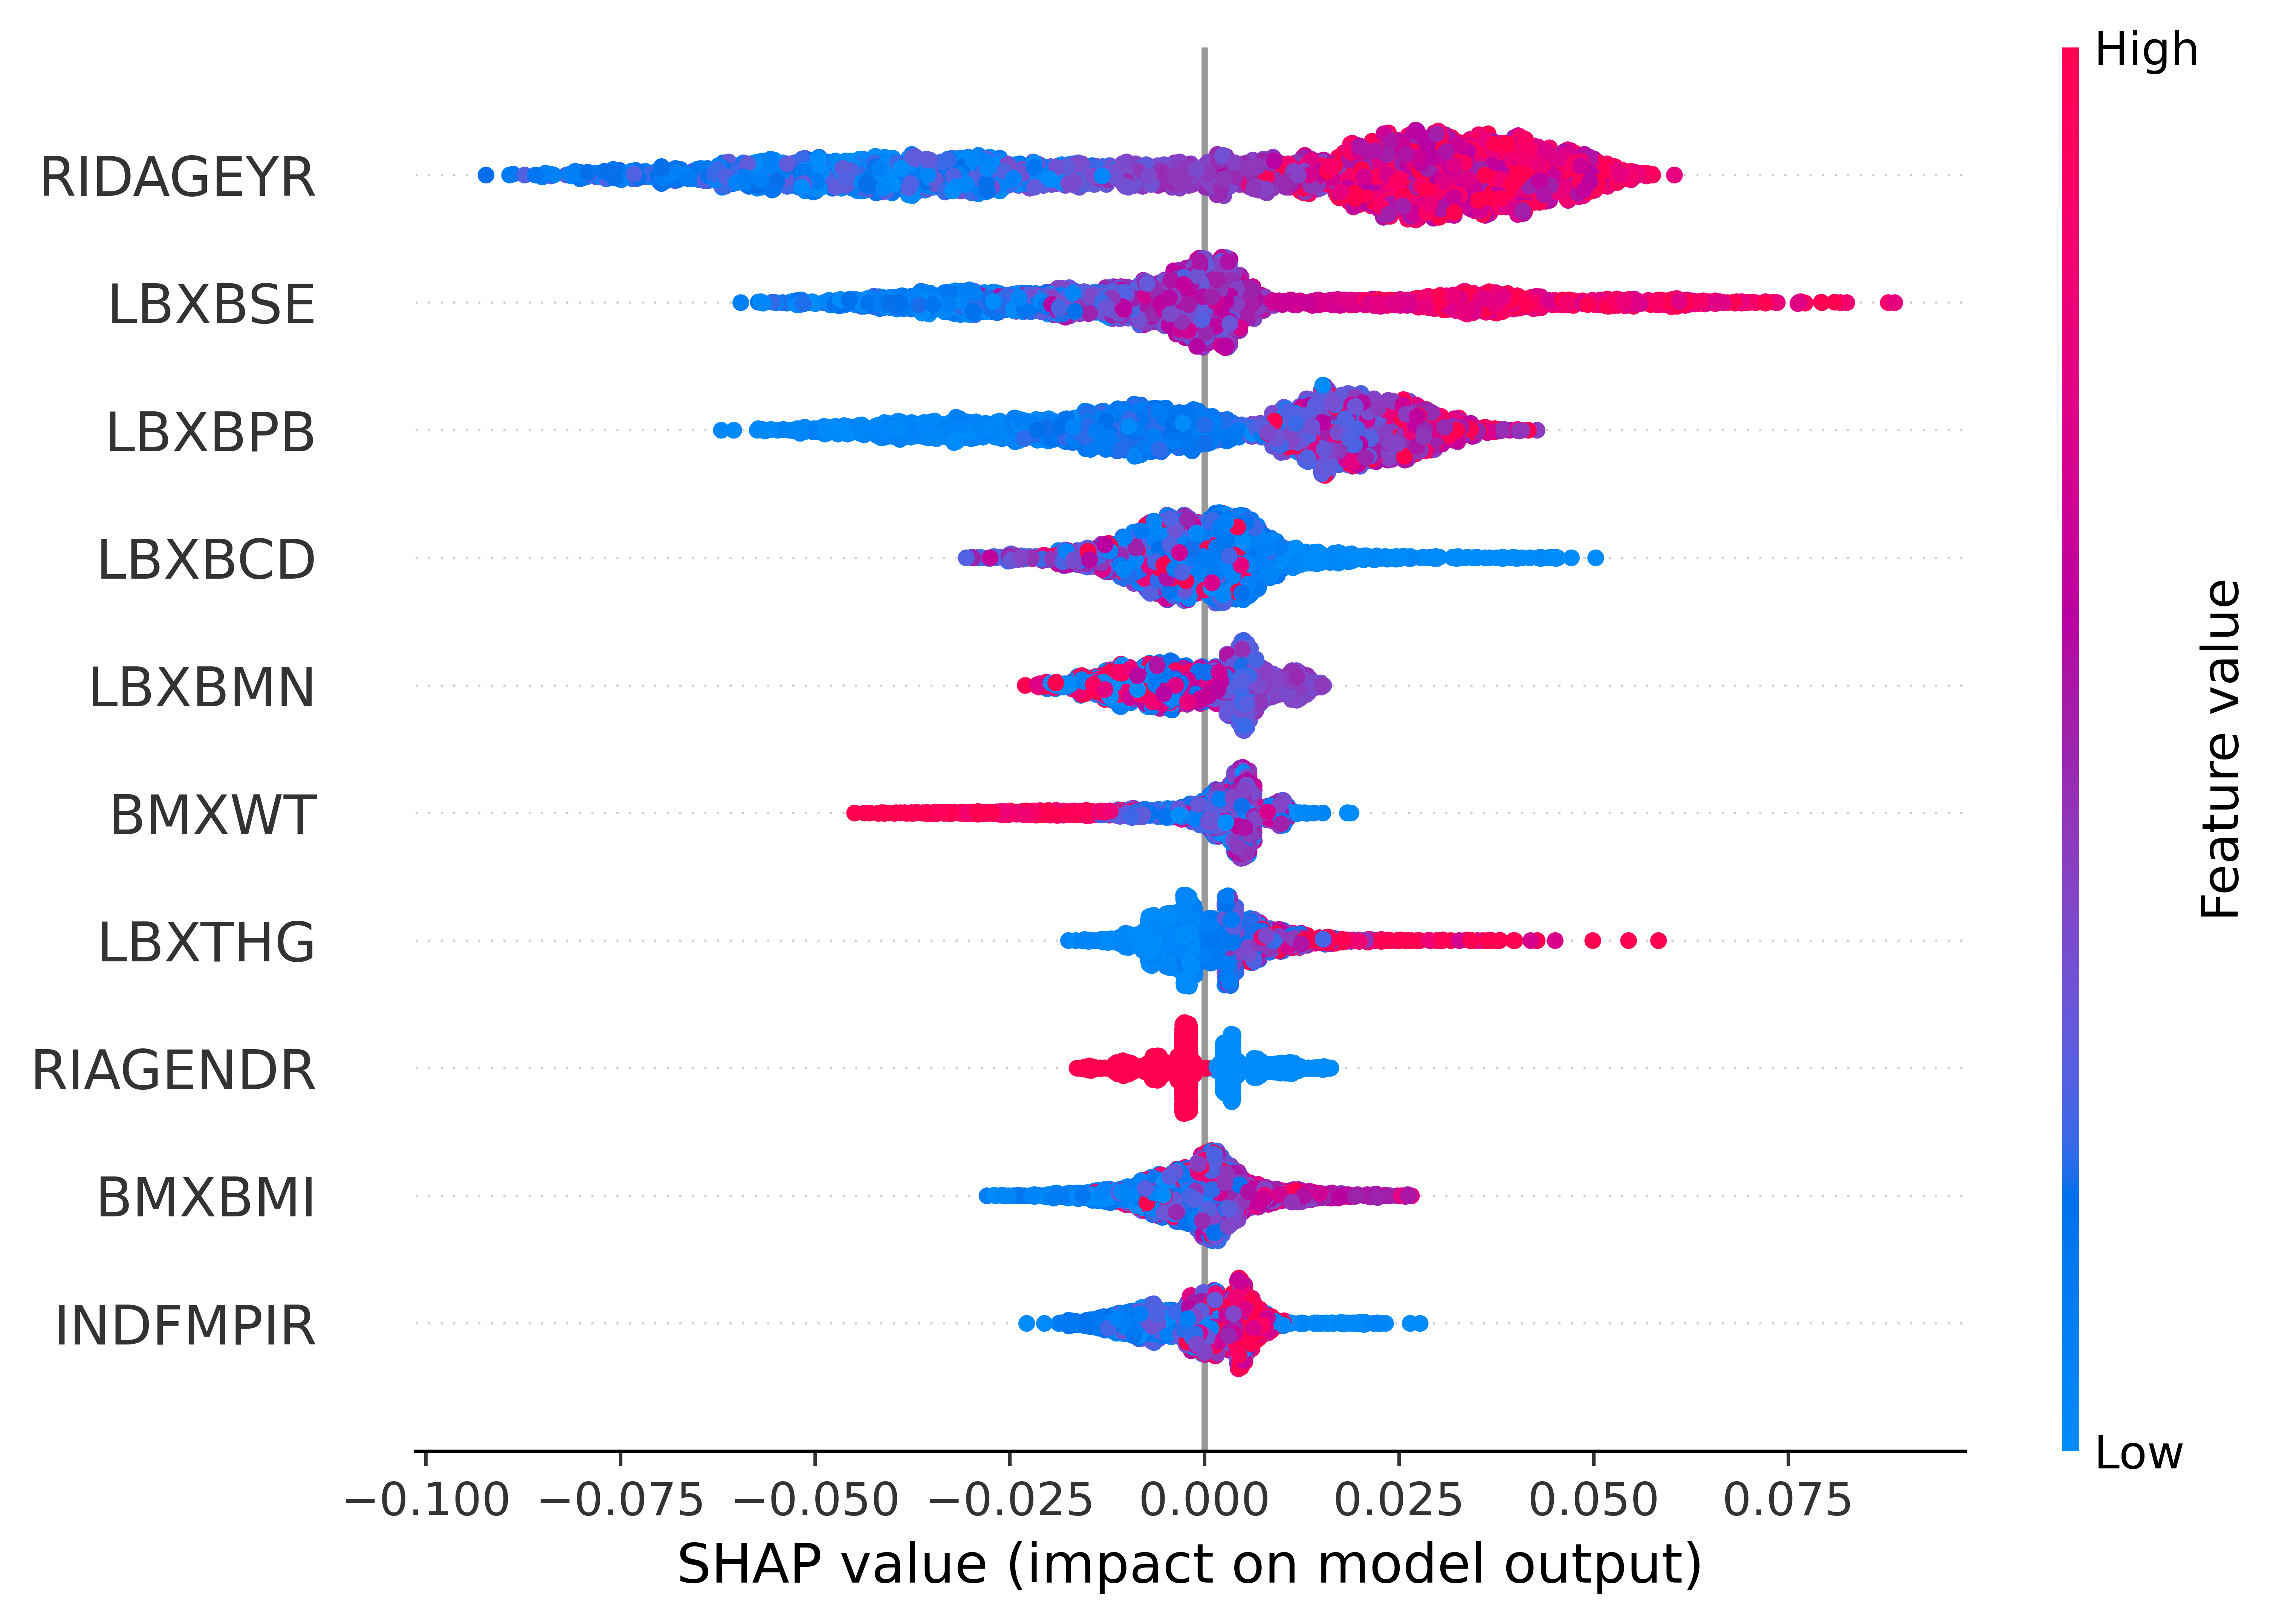
\includegraphics[width=7cm, height=4.8cm]{xgb_mid_beeswarm.png} }}
    \caption{Feature importance for mid group}
\end{figure}

When we are using the middle group subset, for SVM model, the F1 value is 0.525, the balanced accuracy is 0.589, and the ROC-AUC value is 0.623. For XGBoost model, the F1 value is 0.548, the balanced accuracy is 0.5, and the ROC-AUC value is 0.63.

\subsubsection{Old Group}

For the SVM model, the AUC values for each fold ranged from 0.62 to 0.66, with an average AUC of 0.64. For XGB model, the AUC values for each fold ranged from 0.63 to 0.67, with a mean AUC of 0.65. \newpage

\begin{figure}[!ht]
    \centering
    \subfloat[SVM]{{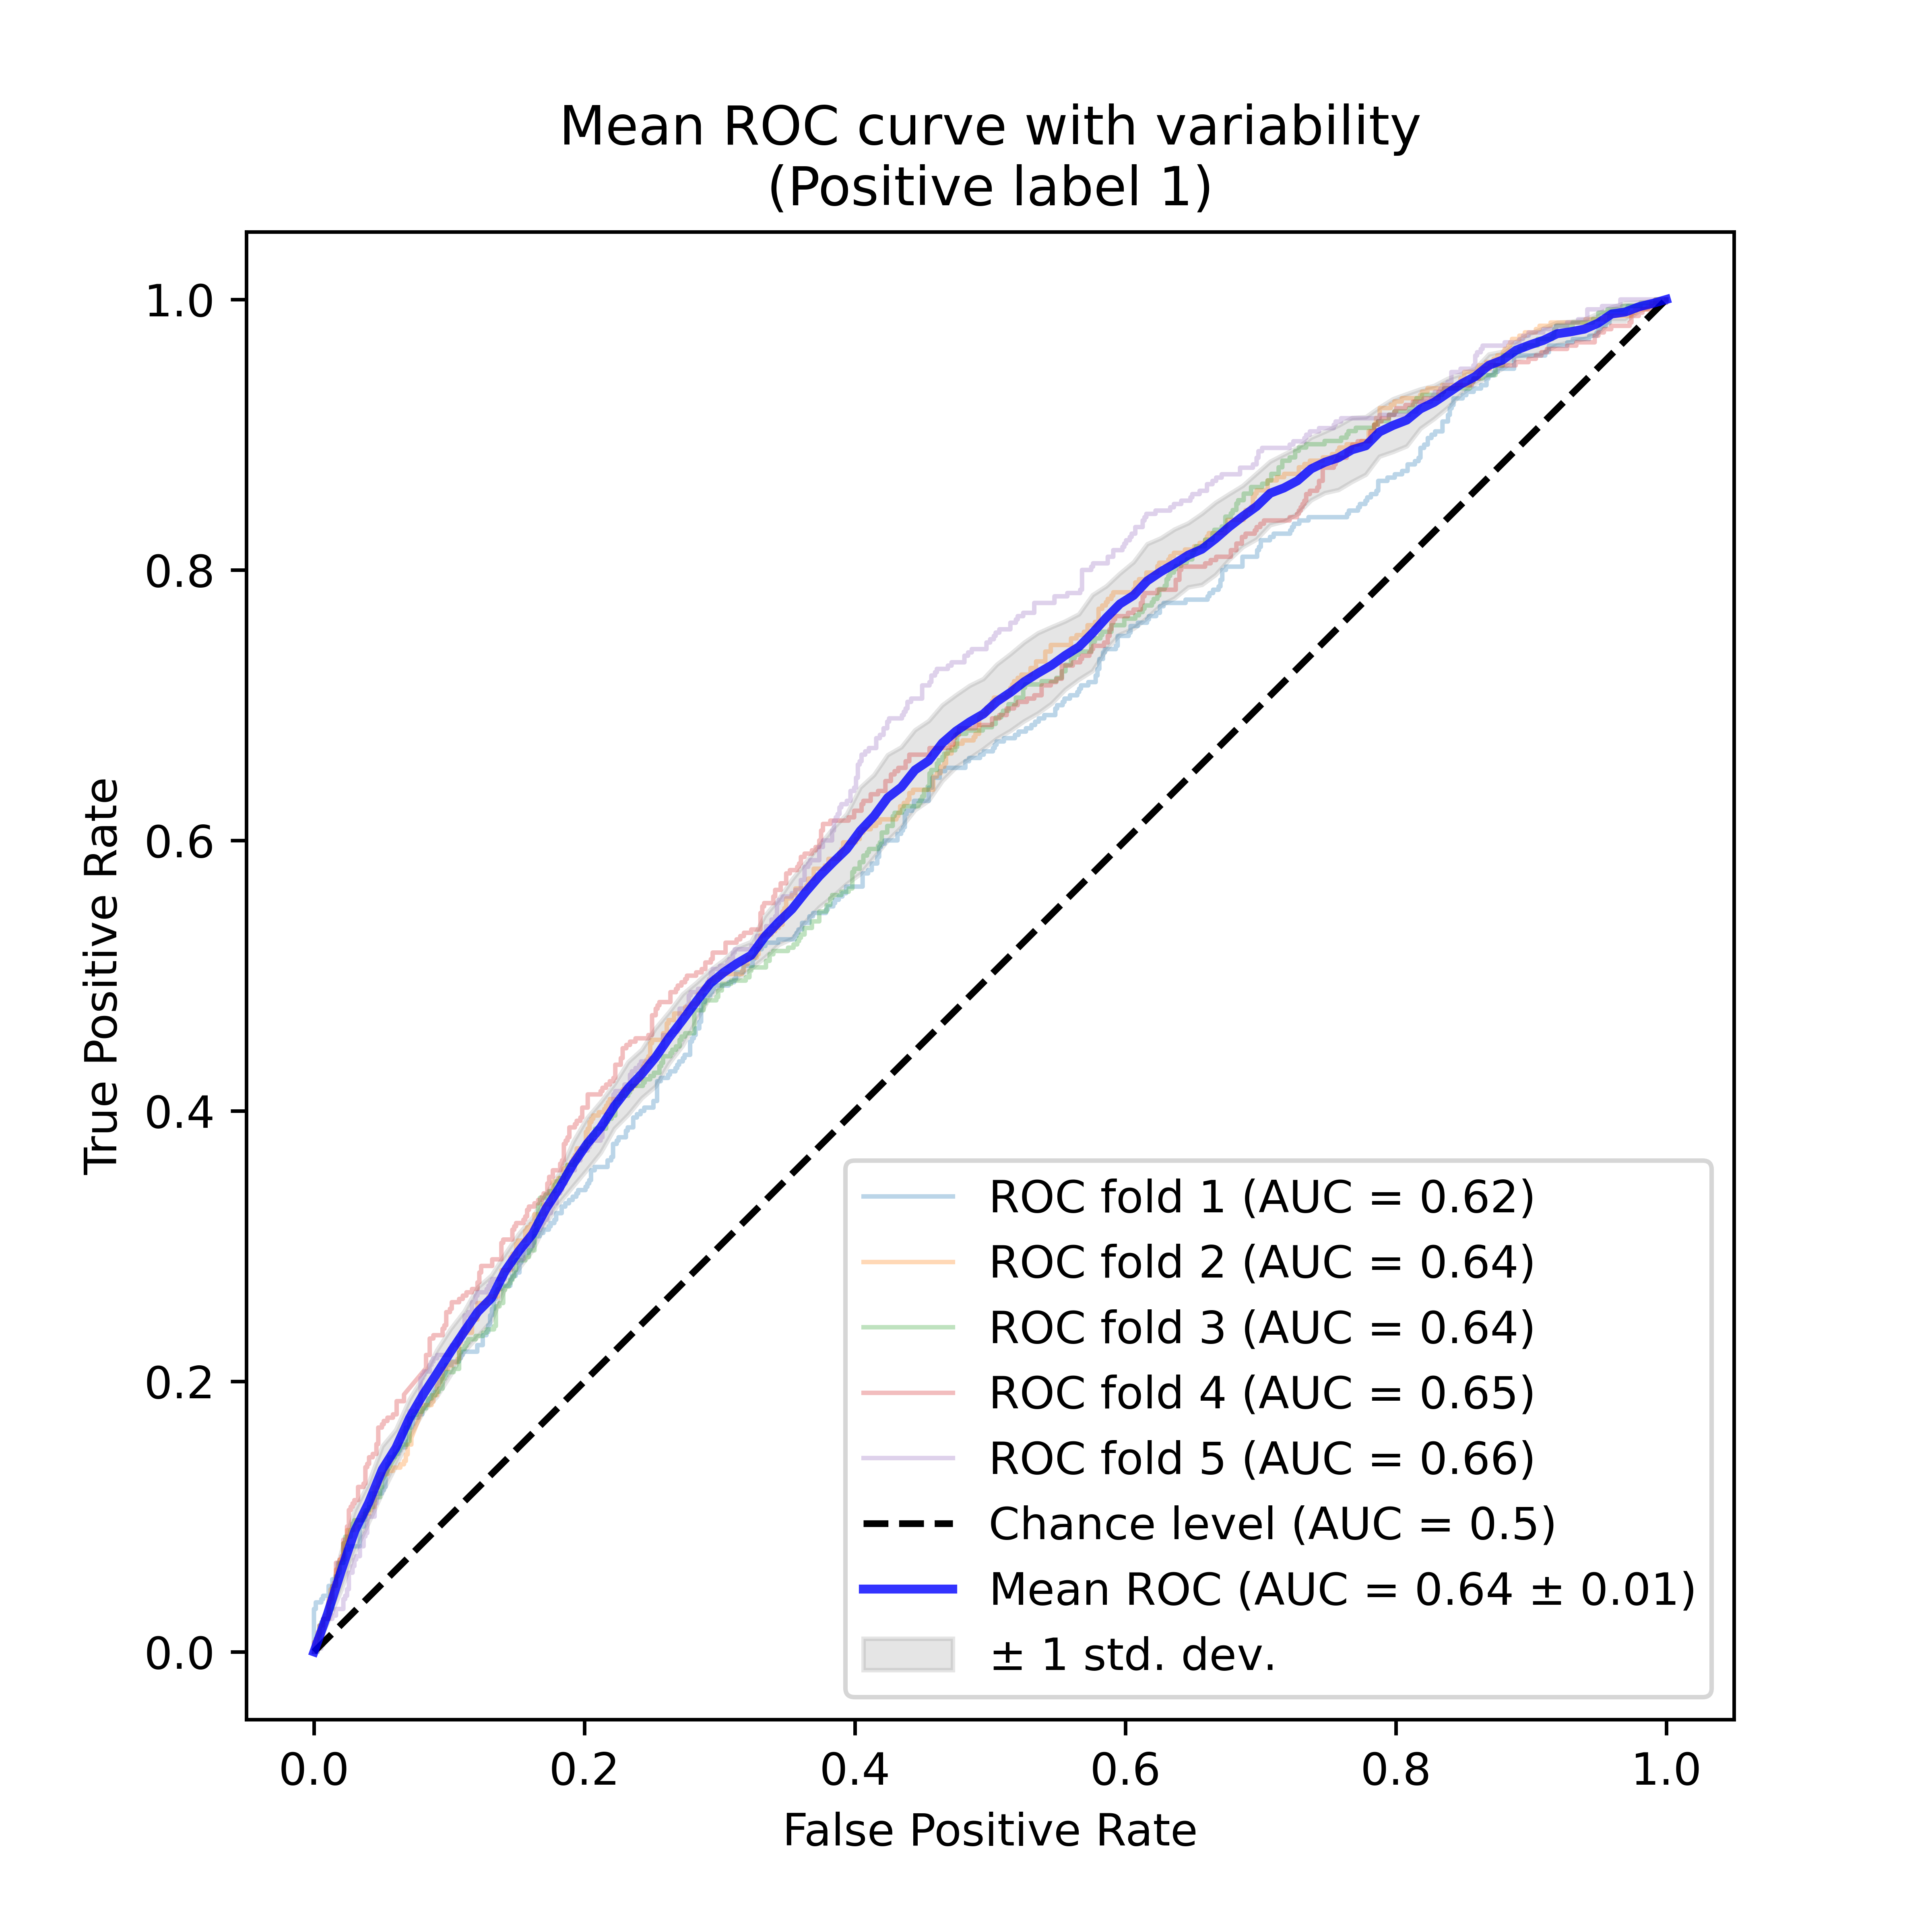
\includegraphics[width=7cm, height=4.8cm]{svm_old_cv_roc.png} }}
    \qquad
    \subfloat[XGB]{{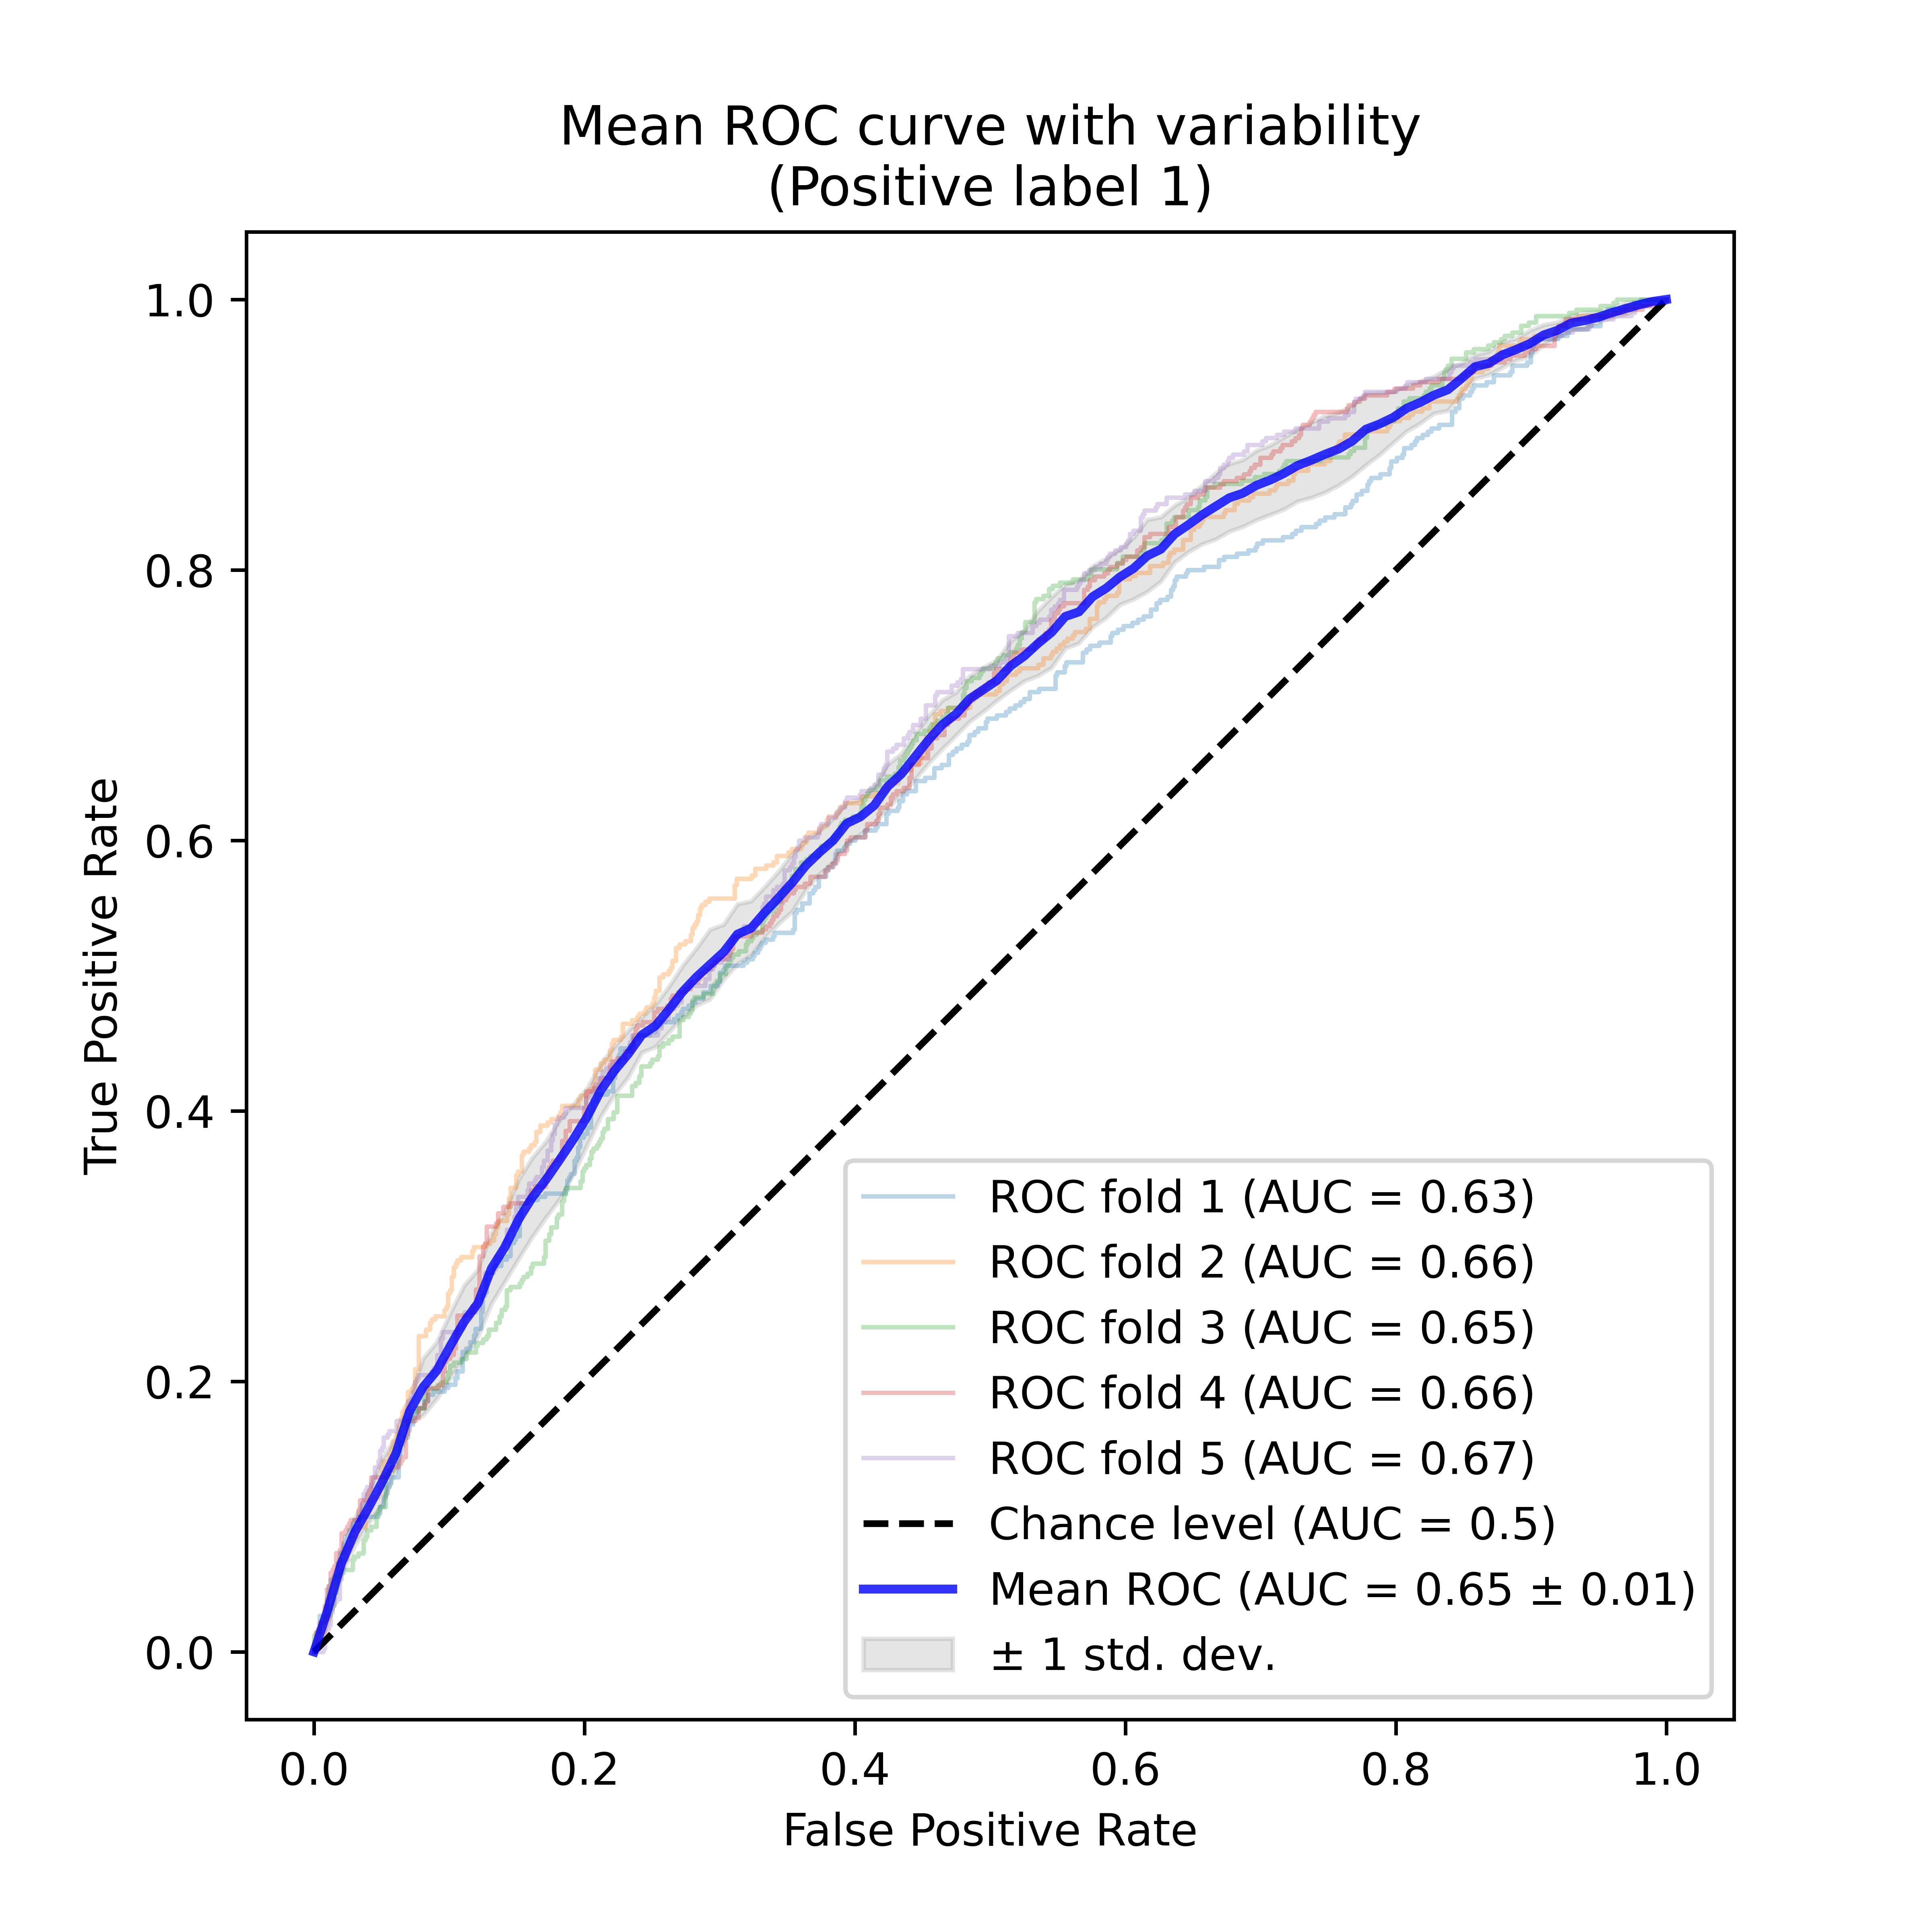
\includegraphics[width=7cm, height=4.8cm]{xgb_old_cv_roc.png} }}
    \caption{Cross validated AUC for old group}
\end{figure}

When we only use the old group of the entire dataset, both the most important features and the least important features change compared to our model using the entire dataset as training data. For SVM model, the most important feature is LBXBPB, and the least important feature is LBXBCD. For the XGB model, the most important feature is RIDAGYR, and the least important feature is BMXBMI. In this case, both models display that females have a higher probability of having high cholesterol levels. In both models, magnesium and cadmium concentrations seem to have mixed effects on the probability of having high cholesterol levels, while other heavy metal concentrations have a positive correlation. Also, it seems that age now has a negative correlation with the probability of having high cholesterol levels.

\begin{figure}[!ht]
    \centering
    \subfloat[SVM]{{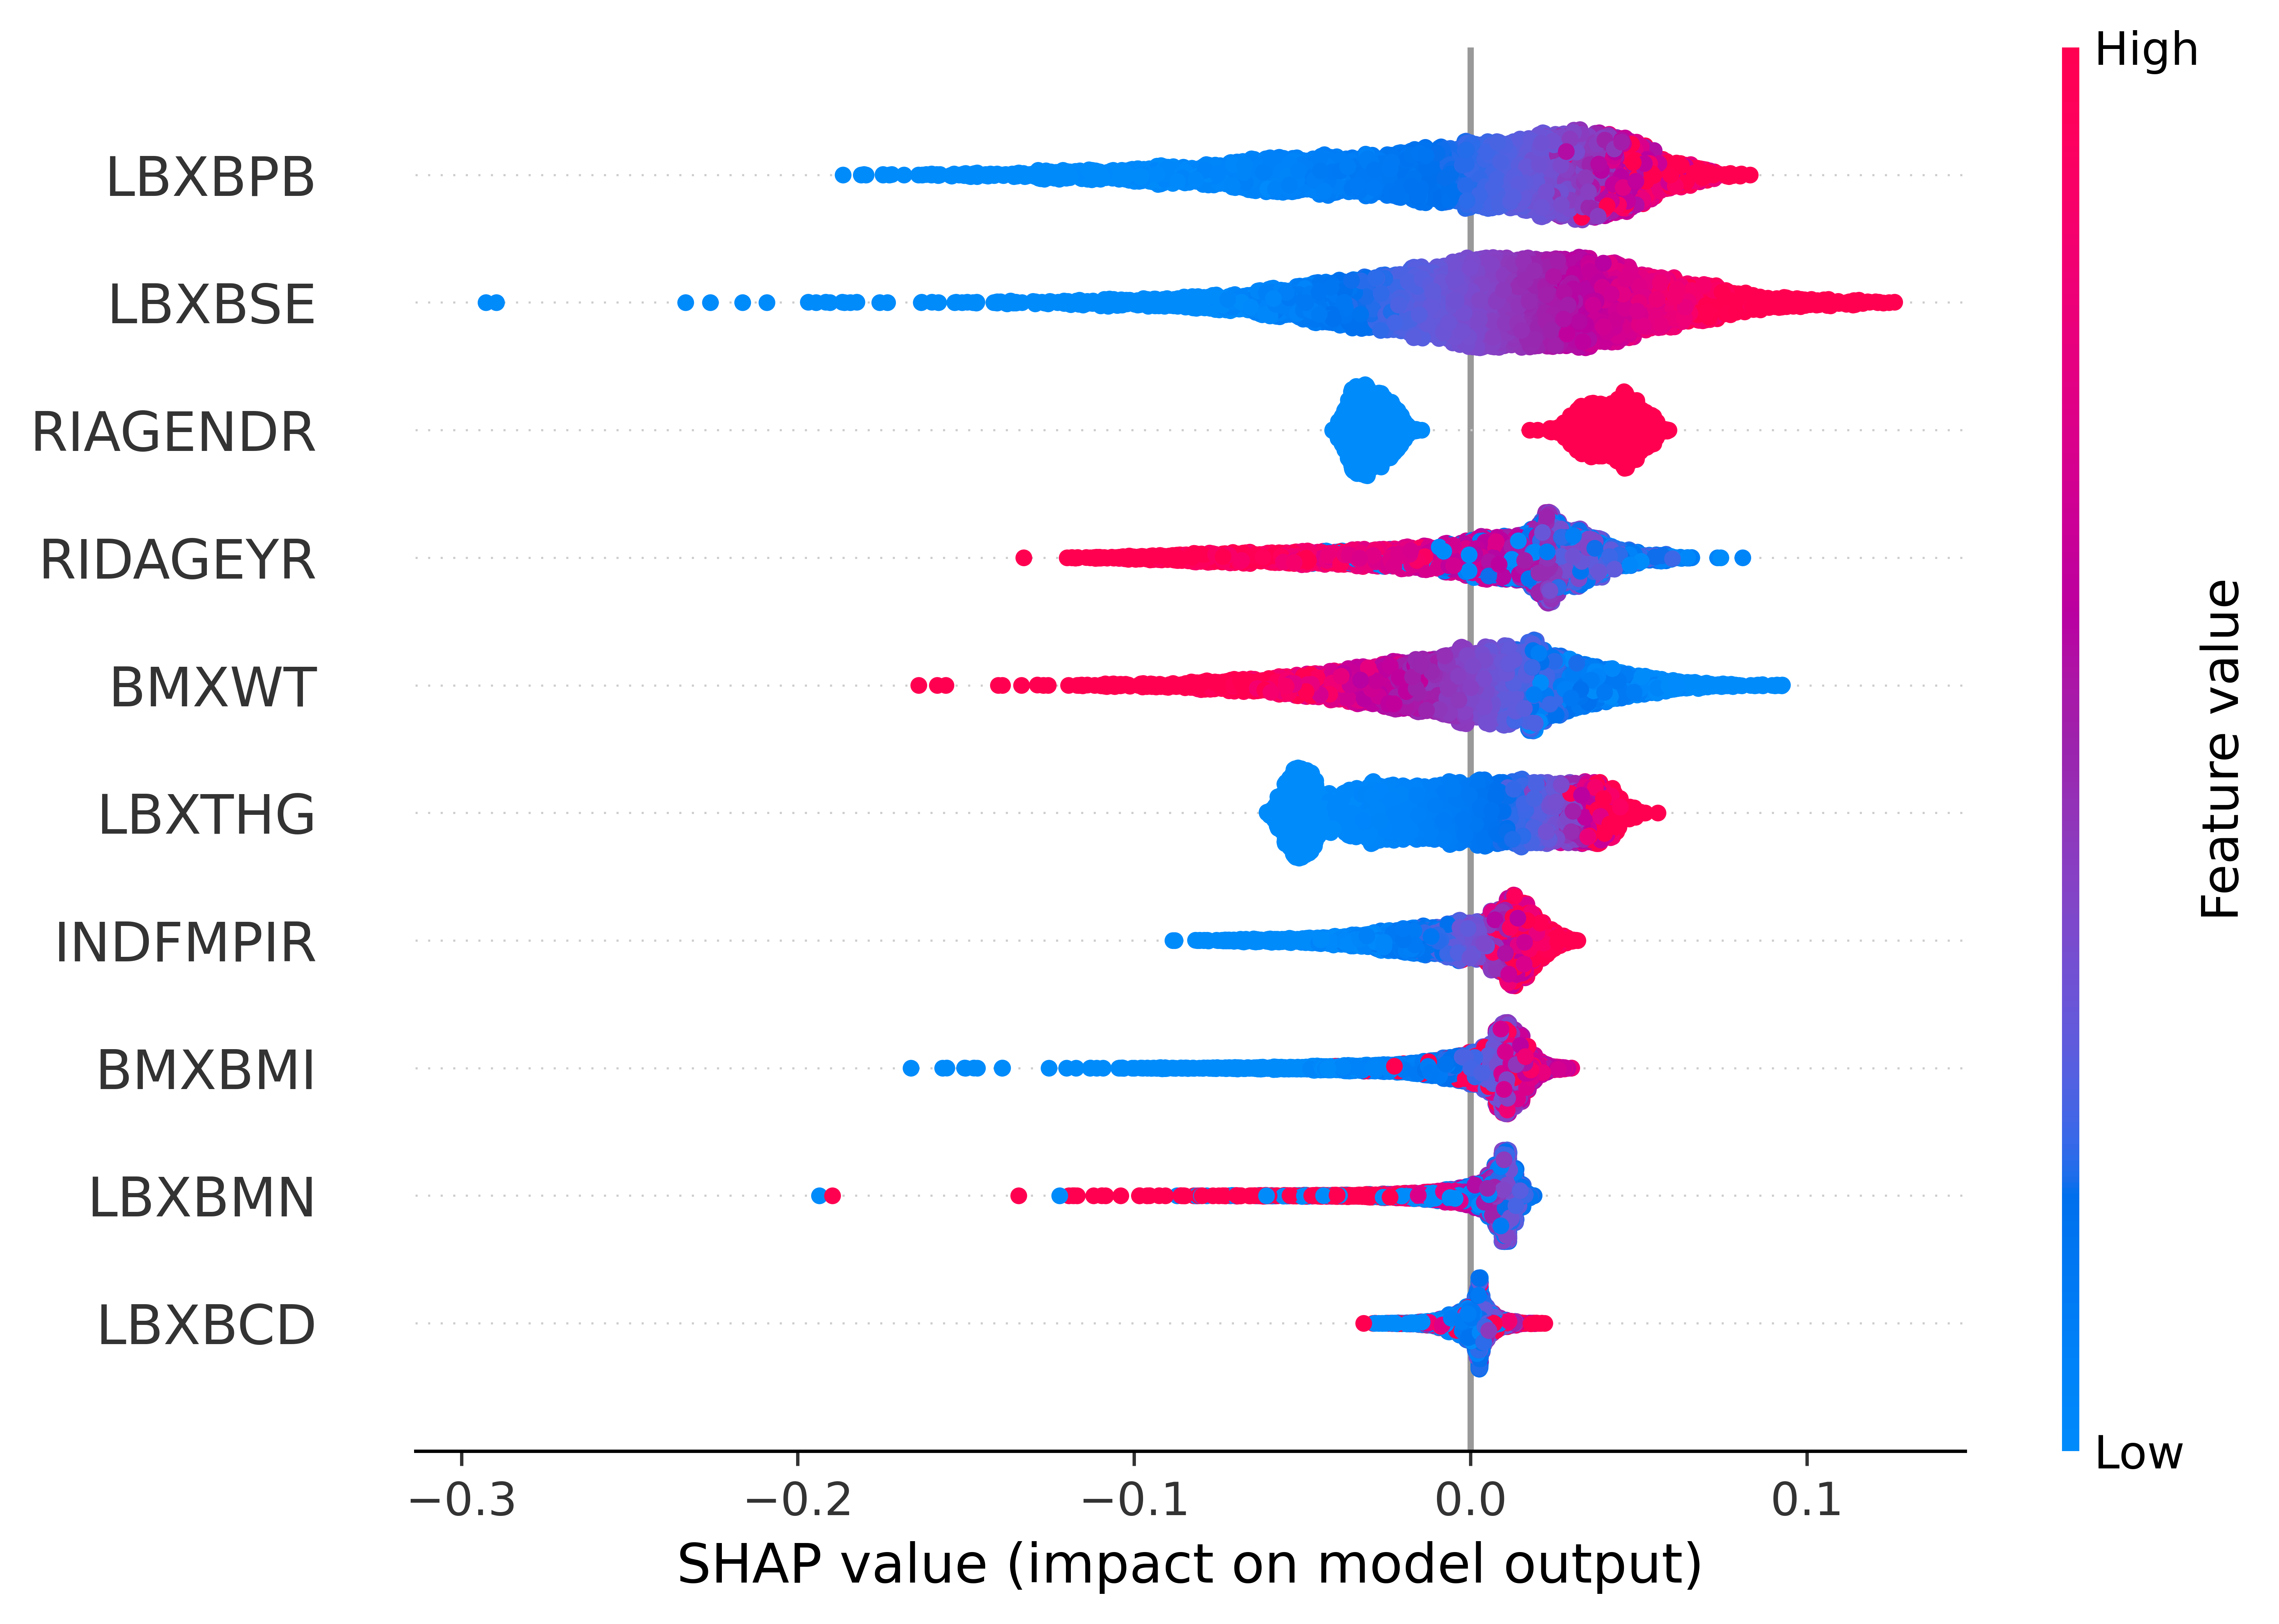
\includegraphics[width=7cm, height=4.8cm]{svm_old_beeswarm.png} }}
    \qquad
    \subfloat[XGB]{{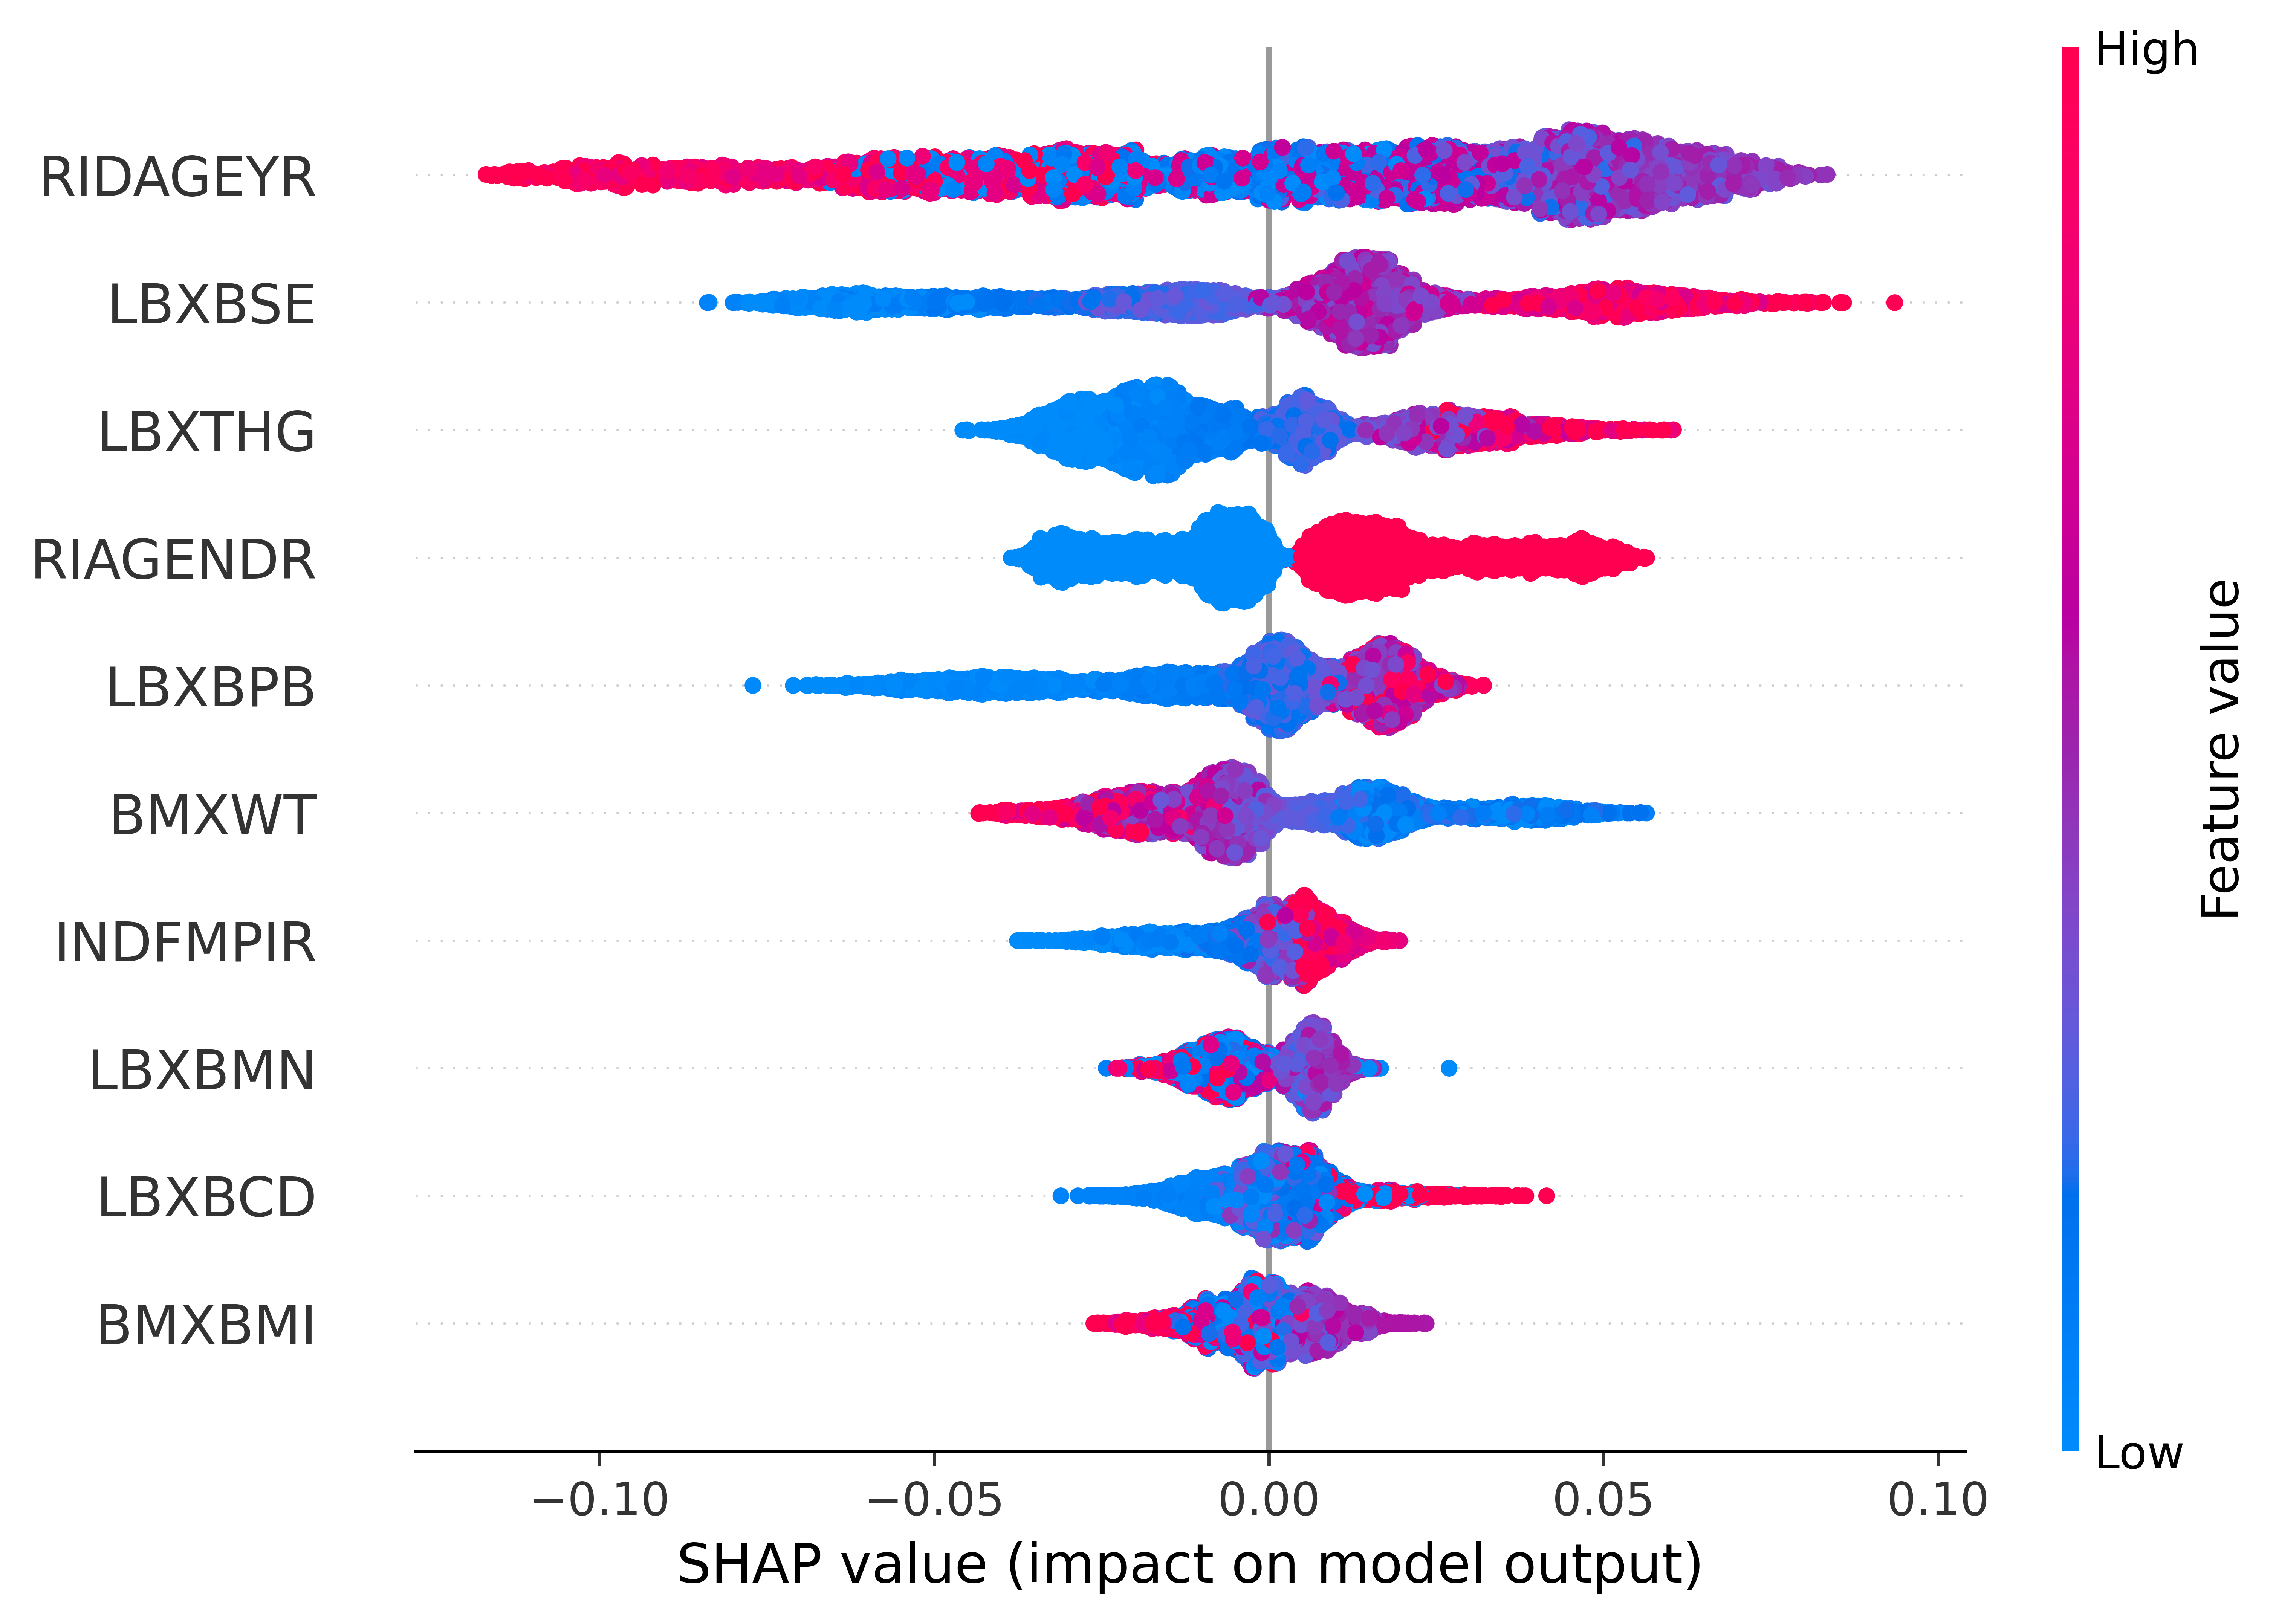
\includegraphics[width=7cm, height=4.8cm]{xgb_old_beeswarm.png} }}
    \caption{Feature importance for old group}
\end{figure}

When we are using the old group subset, for SVM model, the F1 value is 0.528, the balanced accuracy is 0.603, and the ROC-AUC value is 0.641. For XGBoost model, the F1 value is 0.53, the balanced accuracy is 0.507, and the ROC-AUC value is 0.654.

\subsection{Comparative Analysis of Model Performance}

\subsubsection{Overall Performance}
In the analysis of the entire dataset, the XGBoost model outperformed the SVM with an average AUC of 0.75 compared to 0.72 for SVM. This suggests a superior capability of XGBoost in handling complex datasets, likely due to its advanced regularization and tree-based structure, enabling more accurate predictions for high cholesterol risk. Additionally, the consistency of AUC values across different folds in the XGBoost model indicates a better generalization capability to various data subsets.

\subsubsection{Performance Across Age Groups}

When segmenting the dataset by age groups (young, middle-aged, and elderly), notable differences in model performance emerged. In the young age group, both SVM and XGBoost models showed similar AUC values around 0.71. However, for the middle-aged and elderly groups, there was a noticeable performance drop, with average AUC values dipping to 0.62 and 0.63 for SVM, and 0.64 and 0.65 for XGBoost, respectively. This variation might reflect the changing impact of age as a critical variable on cholesterol levels across different age brackets, along with a varying influence of other features in predicting outcomes in these age groups.

\subsubsection{Variation in Feature Importance}

Across the full dataset, both models identified age (RIDAGEYR) as the most significant feature and blood cadmium concentration (LBXBCD) as the least. This highlights the prominence of age in influencing cholesterol levels, while suggesting a minimal impact of blood cadmium concentration.

However, within the age group subsets, changes in feature importance were observed. For instance, in the young group, SVM considered blood cadmium concentration as the least important, whereas XGBoost identified gender (RIAGENDR) as the least significant. Such disparities likely stem from the differing mechanisms within each model in processing the data. In the elderly group, the most significant feature shifted to blood lead concentration (LBXBPB) in SVM, while age continued to dominate in XGBoost. This might indicate that in older age groups, certain biomarkers like blood lead could have a more pronounced impact on cholesterol levels than age itself.

Furthermore, variations in the correlation of certain features with high cholesterol levels were noted across age groups. For example, in the young group, there was a clearer negative correlation of blood magnesium and cadmium concentrations with high cholesterol levels, while in the elderly group, the correlation of age with high cholesterol levels weakened, and other heavy metal concentrations showed a positive correlation.

\section{Conclusions}
In conclusion, we could know more about the correlation between features and the probability of having high cholesterol levels. It seems that age in general have a positive correlation with high cholesterol, but when people get old, getting older seems to be related to lower cholesterol level. This might be explained by people's lifestyles, as people grow older more cholesterol builds up in the body; but when people are very old, usually people ends up living in nursing home or hospitals, which have a stricter diet that can help bring down the cholesterol level. Additionally, it seems that heavy metals such as lead and mercury have a positive correlation with the probability of having high cholesterol levels across all age groups. This makes sense since there are already published research results about those heavy metal's potential health hazards.

However, it is important to note that SHAP values cannot give causal inference and are highly dependent on the model being used. Thus, we should be careful about the interpretation of them provided in the results section, as they might be misleading. Also, since the models' performances are not great, there might be an omitted variable bias, which may lead to some counter-intuitive interpretation of the correlation between features and the probability of having high cholesterol levels. (e.g. the interpretation of gender, body weight, and family income)

\section{Contributions}

All the codes created and used in this project have been uploaded to GitHub, available at the following link: \url{https://github.com/haiming12138/stats415_project/tree/main/final_report}. This report is evenly contributed by each author.

\section{Reproducibility}
To reproduce the same analysis, please see the GitHub repository.
For how to set up the environment, use the shell script automation, make visualization, and find descriptions of each directory and script in the repository, please see this \href{https://github.com/haiming12138/stats415_project/blob/main/final_report/use_guide.md}{document}.

\end{document}